%% ============================================================
%%  Adaptive Neural Control for Mars Rover Wheel Entrapment
%%  Recovery in Granular Terrain
%%
%%  Target: IEEE Transactions on Robotics / IROS 2026
%%  Authors: Meraj Hossain Promit, Chandak Chakma
%%  Supervisors: Md. Jubair Ahmed Sourov, Dr. Sejuti Rahman
%%  University of Dhaka --- Dept. Robotics & Mechatronics Engineering
%% ============================================================

\documentclass[conference]{IEEEtran}

\usepackage[utf8]{inputenc}
\usepackage[T1]{fontenc}
\usepackage{microtype}
\usepackage{amsmath,amssymb,bm}
\usepackage{graphicx}
\graphicspath{{../experiments/regolith_recovery/plots/}{figures/}{../experiments/sim2sim/figs/}}
\usepackage{booktabs}
\usepackage{array}
\usepackage{tabularx}
\usepackage{multirow}
\usepackage{subcaption}
\usepackage{hyperref}
\usepackage{xcolor}
\usepackage{cite}
\usepackage{algorithm}
\usepackage{algpseudocode}
\usepackage{float}
\usepackage{balance}
\usepackage{placeins}
\usepackage{tikz}
\usetikzlibrary{shapes.geometric,arrows.meta,positioning,calc,
                fit,backgrounds,chains}
% \usepackage{fontawesome5}  % not used; disabled to avoid pdflatex font conflicts

% Tighter float spacing to eliminate page whitespace
\setlength{\textfloatsep}{6pt plus 2pt minus 2pt}
\setlength{\floatsep}{6pt plus 2pt minus 2pt}
\setlength{\intextsep}{6pt plus 2pt minus 2pt}
\setlength{\dbltextfloatsep}{6pt plus 2pt minus 2pt}
\setlength{\dblfloatsep}{6pt plus 2pt minus 2pt}
\renewcommand{\topfraction}{0.95}
\renewcommand{\bottomfraction}{0.85}
\renewcommand{\textfraction}{0.05}
\renewcommand{\floatpagefraction}{0.85}
\renewcommand{\dbltopfraction}{0.95}
\renewcommand{\dblfloatpagefraction}{0.85}

\hypersetup{colorlinks=true,linkcolor=blue,citecolor=blue,urlcolor=blue}

%% ── Colours ──────────────────────────────────────────────────────────────────
\definecolor{marsred}{RGB}{150,40,20}
\definecolor{deepblue}{RGB}{40,60,100}
\definecolor{nvgreen}{HTML}{76B900}
\definecolor{boxgray}{RGB}{248,248,248}
\definecolor{headerblue}{RGB}{50,80,130}
\definecolor{accentorange}{RGB}{200,100,30}
\definecolor{softgreen}{RGB}{60,140,60}
\definecolor{softpurple}{RGB}{100,60,150}
\definecolor{softcyan}{RGB}{40,130,150}
\definecolor{lightblue}{RGB}{220,235,250}
\definecolor{lightorange}{RGB}{255,235,210}
\definecolor{lightred}{RGB}{255,220,220}
\definecolor{lightgreen}{RGB}{220,245,220}
\definecolor{MarsRust}{HTML}{C1440E}
\definecolor{ArcticTeal}{HTML}{00897B}
\definecolor{AccentGreen}{HTML}{2E7D32}
\definecolor{WarnOrange}{HTML}{E65100}
\definecolor{SandGold}{HTML}{A67C00}
\definecolor{NebulaPurple}{HTML}{4A3F8C}
\definecolor{CosmicBlue}{HTML}{E9ECEF}
\definecolor{TextLight}{HTML}{2D3748}
\definecolor{CardBg}{HTML}{F4F6F9}
\definecolor{DimText}{HTML}{6C757D}
\definecolor{StarWhite}{HTML}{111111}

% ══════════════════════════════════════════════════════════════
\begin{document}

\title{Adaptive Neural Control for Mars Rover\\
       Wheel Entrapment Recovery in Granular Terrain}

\IEEEoverridecommandlockouts
\author{Meraj Hossain Promit\IEEEauthorrefmark{1},
        Chandak Chakma\IEEEauthorrefmark{1},
        Dr.~Sejuti Rahman\IEEEauthorrefmark{2},
        and Md.~Jubair Ahmed Sourov\IEEEauthorrefmark{2}%
  \thanks{All authors are with the Department of Robotics and Mechatronics
          Engineering, University of Dhaka, Dhaka, Bangladesh.
          E-mail: \{merajhossainpromit, chandakchakma\}@du.ac.bd.}%
  \thanks{\IEEEauthorrefmark{1}Student Author.\quad
          \IEEEauthorrefmark{2}Supervisor.}%
}

\maketitle

% ── Abstract ─────────────────────────────────────────────────────────────────
\begin{abstract}
Wheel entrapment in granular regolith is one of the most critical failure modes
for planetary rovers, as demonstrated by the permanent loss of NASA's Spirit rover
in 2009. We present an autonomous entrapment recovery system for a 6-wheel
rocker-bogie Mars rover trained entirely in simulation using deep reinforcement
learning (DRL). Our primary contribution is the first coupling of Newton Material
Point Method (MPM) granular physics with MuJoCo rigid-body dynamics inside Isaac
Lab's DirectRLEnv for RL-based entrapment recovery, producing physically accurate
wheel--soil interaction under Martian gravity ($3.72\,\text{m/s}^2$). A recurrent
policy (PPO+GRU, hidden size 256) with an asymmetric actor--critic --- actor
observes a 29-dimensional proprioceptive vector, critic additionally reads 8
privileged simulator features --- is trained for 300\,000 policy steps across 16
parallel environments on a single workstation with an NVIDIA RTX 5070\,Ti. After
training, the policy attains an \textbf{86.9\,\% episode success rate}, with
episodic return rising monotonically from $-20.7$ to $+35.1$ (isotonic-regression
envelope) while policy entropy remains above $0.5$\,nats throughout, confirming no
premature convergence. Emergent behaviours include coordinated rocking and
asymmetric wheel-steering sequences that were never explicitly scripted. We
further validate the system in a sim-to-sim A$\to$B navigation scenario: a
dual-mode entrapment detector transfers control between a PD navigation brain and
the trained escape policy, and the same policy handles arbitrary GPS bearings
through omnidirectional heading generalisation, enabling \emph{zero-shot}
goal-directed recovery. We further demonstrate cross-engine transfer by
evaluating the exported ONNX policy on Project Chrono
(\texttt{ChSystemNSC} complementarity solver) with a morphologically distinct
Curiosity rover (899\,kg, 0.25\,m wheel radius) over a rigid flat surface with
randomised low friction ($\mu\in[0.10,0.35]$), achieving a \textbf{47.3\%}
recovery rate (95\% CI [39.3\%, 55.3\%]) across 150 zero-shot trials---without
any fine-tuning or parameter adaptation. To our knowledge, this is the first
DRL-based entrapment
recovery system to employ full granular MPM coupling for a rocker-bogie platform
under Mars gravity. Project repository:
\href{https://github.com/promit7473/regolith-entrapment-rl.git}{\textcolor{nvgreen}{\nolinkurl{https://github.com/promit7473/regolith-entrapment-rl.git}}}.
\end{abstract}

\begin{IEEEkeywords}
planetary rovers, wheel entrapment, reinforcement learning, granular simulation,
Material Point Method, PPO, GRU, Mars, regolith, curriculum learning,
sim-to-sim validation, dual-brain architecture
\end{IEEEkeywords}

\begin{figure}[!t]
  \centering
  \resizebox{\columnwidth}{!}{%
    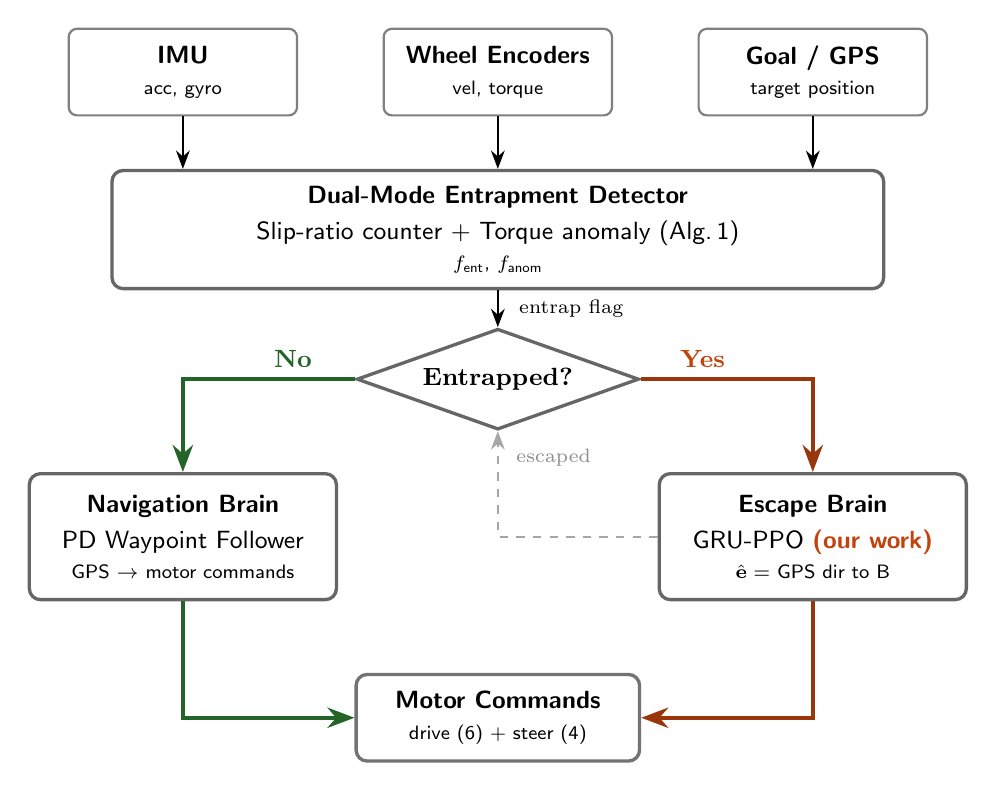
\begin{tikzpicture}[
      >=Stealth, font=\sffamily\small,
      sbox/.style={rectangle, draw=black!50, thick, rounded corners=3pt,
                   fill=white, align=center, minimum width=2.9cm,
                   minimum height=1.1cm},
      dbox/.style={rectangle, draw=black!60, line width=1.2pt,
                   rounded corners=4pt, fill=white, align=center,
                   minimum width=9.8cm, minimum height=1.5cm},
      nbox/.style={rectangle, draw=black!60, line width=1.2pt,
                   rounded corners=4pt, fill=white, align=center,
                   minimum width=3.9cm, minimum height=1.6cm},
      ebox/.style={rectangle, draw=black!60, line width=1.2pt,
                   rounded corners=4pt, fill=white, align=center,
                   minimum width=3.9cm, minimum height=1.6cm},
      mbox/.style={rectangle, draw=black!55, line width=1.2pt,
                   rounded corners=4pt, fill=white, align=center,
                   minimum width=5.5cm, minimum height=1.1cm},
      dec/.style={diamond, draw=black!60, line width=1.2pt,
                  fill=none, align=center, aspect=2.8,
                  font=\small\bfseries},
      a/.style={-Stealth, thick},
      ga/.style={-Stealth, line width=1.5pt, color=AccentGreen!80!black},
      ra/.style={-Stealth, line width=1.5pt, color=MarsRust!80!black},
      da/.style={-Stealth, thick, dashed, color=black!35},
    ]
      \node[sbox] (imu) at (-4,  5.6) {\textbf{IMU}\\{\scriptsize acc, gyro}};
      \node[sbox] (enc) at ( 0,  5.6) {\textbf{Wheel Encoders}\\
                                       {\scriptsize vel, torque}};
      \node[sbox] (gps) at ( 4,  5.6) {\textbf{Goal / GPS}\\
                                       {\scriptsize target position}};

      \node[dbox] (det) at (0, 3.6) {%
        \textbf{Dual-Mode Entrapment Detector}\\[2pt]
        {\small Slip-ratio counter + Torque anomaly (Alg.\,1)}\\
        {\scriptsize $f_\text{ent}$, $f_\text{anom}$}};

      \node[dec] (dmd) at (0, 1.7) {\textbf{Entrapped?}};

      \node[nbox] (nav) at (-4, -0.3) {%
        \textbf{Navigation Brain}\\[2pt]
        {\small PD Waypoint Follower}\\
        {\scriptsize GPS $\to$ motor commands}};

      \node[ebox] (esc) at (4, -0.3) {%
        \textbf{Escape Brain}\\[2pt]
        {\small GRU-PPO {\color{MarsRust}\textbf{(our work)}}}\\
        {\scriptsize $\hat{\mathbf{e}} = $ GPS dir to B}};

      \node[mbox, minimum width=3.6cm] (mot) at (0, -2.6) {%
        \textbf{Motor Commands}\\{\scriptsize drive (6) + steer (4)}};

      \draw[a]  (imu.south) -- (imu|-det.north);
      \draw[a]  (enc.south) -- (det.north);
      \draw[a]  (gps.south) -- (gps|-det.north);
      \draw[a]  (det.south) -- (dmd.north)
                node[midway, right=4pt, font=\scriptsize] {entrap flag};
      \draw[ga] (dmd.west)  -| (nav.north)
                node[pos=0.18, above, font=\small\bfseries,
                     text=AccentGreen!80!black] {No};
      \draw[ra] (dmd.east)  -| (esc.north)
                node[pos=0.18, above, font=\small\bfseries,
                     text=MarsRust] {Yes};
      \draw[ga] (nav.south) |- (mot.west);
      \draw[ra] (esc.south) |- (mot.east);
      \draw[da] (esc.west)  -- (0,-0.3) -- (dmd.south)
                node[pos=0.75, right=3pt, font=\scriptsize,
                     text=black!45] {escaped};
    \end{tikzpicture}%
  }
  \caption{Dual-brain on-board architecture. During normal traversal the PD
    Navigation Brain drives toward GPS goal B; the dual-mode entrapment detector
    triggers handover to the GRU-PPO Escape Brain when $f_\text{ent}$ fires.
    Escape direction is set to the GPS bearing toward B (zero-shot
    generalisation). After escape, control returns to navigation automatically.}
  \label{fig:dual_brain}
\end{figure}

% ══════════════════════════════════════════════════════════════
\section{Introduction}
\label{sec:intro}

On May~1, 2009, NASA's Spirit rover drove into soft sulfate-rich regolith and
never moved again~\cite{arvidson2011spirit}. Eight months of carefully scripted
extraction commands, constrained by a 4--24 minute round-trip communication delay,
failed to free the vehicle. Spirit had no on-board capability to detect or respond
to the entrapment autonomously, \emph{it had no way to save itself}.

Wheel entrapment in granular regolith is a systemic risk for Mars exploration.
Rovers operate over extensive dune fields, impact crater interiors filled with
fine regolith, and wind-blown sand deposits. The rocker-bogie suspension, while
excellent on rocky terrain, can cause individual wheels to sink disproportionately
in loose material. As missions extend beyond planned durations, Spirit operated
for $5\times$ its planned 90-sol lifetime, Opportunity for $55\times$, the
probability of encountering entrapment-prone terrain grows monotonically.

The fundamental operational constraint is autonomy: one-way communication
latencies of up to 24 minutes make real-time teleoperation impossible during
entrapment events. Any practical recovery system must operate entirely on-board,
detecting entrapment and executing recovery manoeuvres without ground intervention.

Prior DRL-based recovery work~\cite{bi2026escape,jain2019} addresses either
4-wheel skid-steered platforms in rigid terrain or simplified soil models. No
existing method trains a recovery policy for a \emph{6-wheel rocker-bogie rover}
in \emph{physics-accurate granular simulation} under \emph{Mars gravity}. These
three factors jointly determine the problem's difficulty: granular sinkage
progresses over several seconds (requiring memory), Mars gravity reduces
wheel--soil traction by 62\%, and rocker-bogie kinematics create coupled sinkage
dynamics across axles that demand a larger, more expressive action space.

\textbf{Contributions.} This paper makes five contributions:
\begin{enumerate}
  \item \textbf{Physics stack.} The first coupling of Newton MPM granular
        physics with MuJoCo rigid-body dynamics inside Isaac Lab's
        DirectRLEnv for DRL-based entrapment recovery on a rocker-bogie
        platform under Mars gravity. The coupling is two-way: wheel SDF
        geometry displaces sand particles, and the resulting particle impulses
        feed back as external forces on the rover body each physics substep.
  \item \textbf{Policy architecture.} A recurrent PPO+GRU policy with an
        asymmetric actor--critic (29D actor, 37D privileged critic), a
        9-term world-frame-projected shaped reward including an explicit
        reverse penalty that eliminates the backward-drift local optimum, and
        a competence-gated curriculum over sinkage depth that is
        symmetric-fail-closed on an empty rolling window.
  \item \textbf{Omnidirectional escape.} Training with per-episode uniformly
        random escape headings enables \emph{zero-shot} GPS-directed recovery
        at deployment without heading-specific fine-tuning; the body-frame
        policy is heading-agnostic and receives its escape bearing exogenously
        at runtime.
  \item \textbf{Dual-brain deployment.} A sim-to-sim A$\to$B navigation harness
        that integrates a PD navigation brain, a dual-mode entrapment
        detector (slip-ratio AND-gate + leaky torque-anomaly OR-gate), and
        the trained recovery policy, with automatic handoff in both
        directions and quantitative comparison against a no-recovery
        baseline.
  \item \textbf{Cross-engine sim-to-sim validation.} The trained ONNX policy
        is evaluated zero-shot on Project Chrono
        (\texttt{ChSystemNSC} non-smooth complementarity solver) with a
        morphologically distinct Curiosity rover (NASA MSL analogue, 899\,kg,
        0.25\,m wheel radius, 25$\times$ the AAU rover mass) over a rigid flat
        surface with randomised low friction ($\mu\in[0.10,0.35]$). The
        experiment simultaneously stresses three transfer axes: rigid-solver
        gap (Newton MPM $\to$ Chrono NSC), terrain-physics-class gap (continuum
        elasto-plastic MPM $\to$ rigid contact), and rover morphology gap (AAU
        35\,kg $\to$ Curiosity 899\,kg). Achieving \textbf{47.3\%} recovery
        (95\% CI [39.3\%, 55.3\%]) across 150 zero-shot trials demonstrates
        that the learned recovery strategy generalises beyond training-simulator
        specifics.
\end{enumerate}

% ══════════════════════════════════════════════════════════════
%  FULL-WIDTH FIGURE: System Overview  (two-column)
% ══════════════════════════════════════════════════════════════
\begin{figure*}[t]
  \centering
  \resizebox{0.86\textwidth}{!}{%
    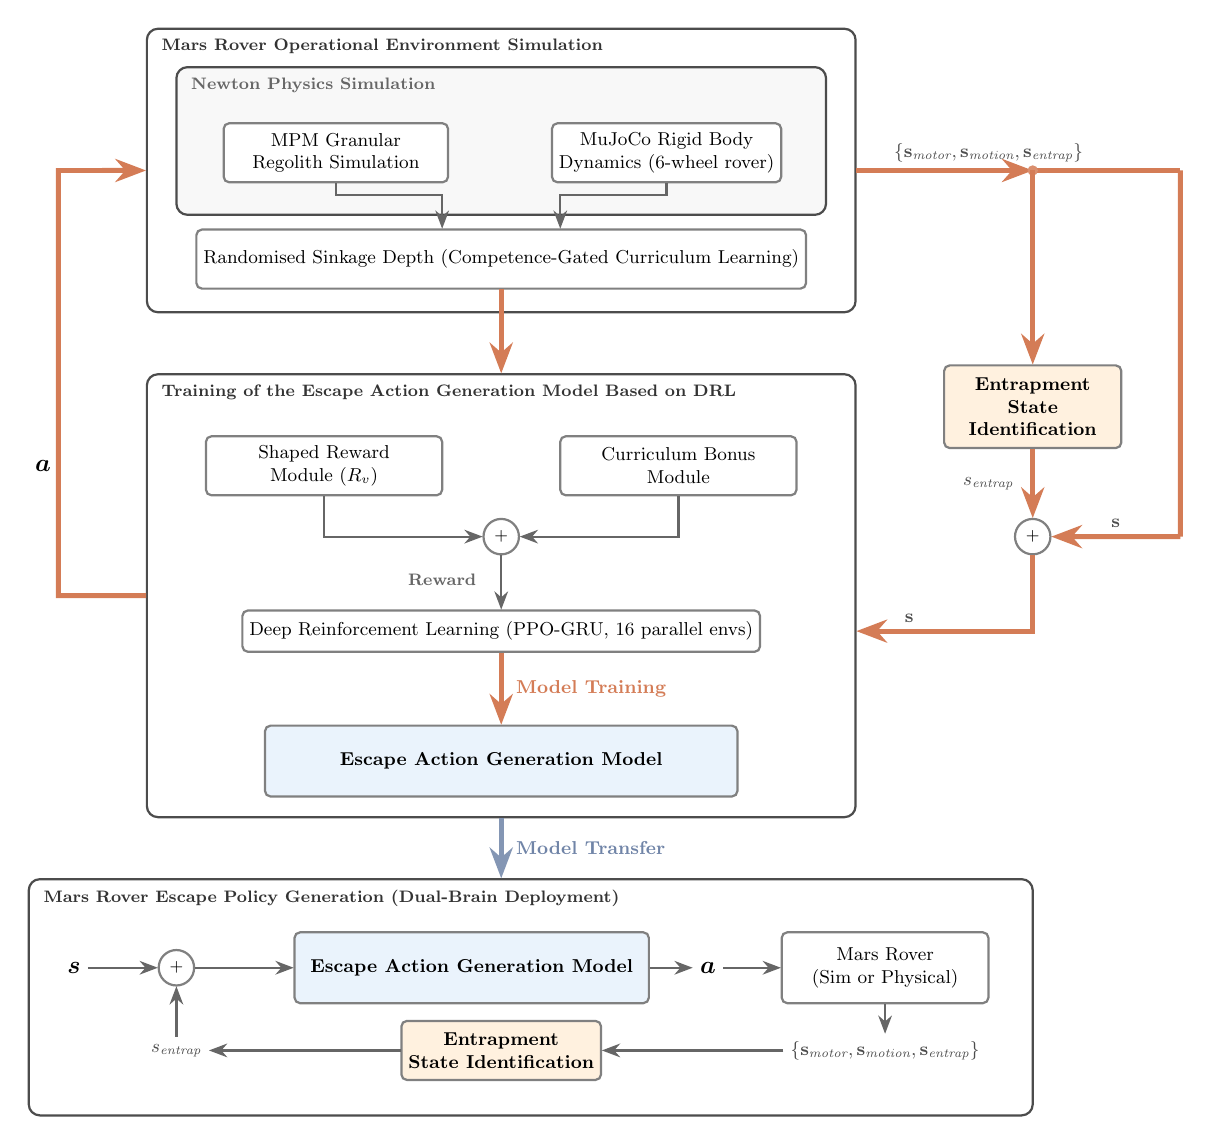
\begin{tikzpicture}[
      scale=0.75, transform shape,
      outerbox/.style={rectangle, draw=black!70, thick, rounded corners=4pt,
                       inner sep=10pt},
      innerbox/.style={rectangle, draw=black!50, thick, fill=white,
                       minimum height=1cm, minimum width=3.8cm,
                       align=center, font=\small, rounded corners=2pt},
      orangebox/.style={innerbox, fill=lightorange!70, font=\small\bfseries},
      bluebox/.style={innerbox, fill=lightblue!60, font=\small\bfseries},
      redarrow/.style={-Stealth, line width=1.8pt, color=MarsRust!70},
      bluearrow/.style={-Stealth, line width=1.8pt, color=headerblue!60},
      arrow/.style={-Stealth, thick, color=black!60},
      circnode/.style={draw=black!50, circle, thick, minimum size=0.6cm,
                       inner sep=0pt, font=\footnotesize},
      every node/.style={font=\small}
    ]
      %% Training environment block
      \node[outerbox, fill=white, minimum width=12cm, minimum height=4.8cm]
            (simbox) at (0, 12.5) {};
      \node[font=\footnotesize\bfseries, anchor=north west, text=black!80]
            at ([xshift=4pt, yshift=-2pt]simbox.north west)
            {Mars Rover Operational Environment Simulation};
      \node[outerbox, fill=boxgray, minimum width=11cm, minimum height=2.5cm]
            (physbox) at (0, 13.0) {};
      \node[font=\footnotesize\bfseries, anchor=north west, text=black!60]
            at ([xshift=4pt, yshift=-2pt]physbox.north west)
            {Newton Physics Simulation};
      \node[innerbox] (mpm)   at (-2.8, 12.8) {MPM Granular\\Regolith Simulation};
      \node[innerbox] (rigid) at ( 2.8, 12.8) {MuJoCo Rigid Body\\Dynamics (6-wheel rover)};
      \node[innerbox, minimum width=7cm] (terrain) at (0, 11.0)
            {Randomised Sinkage Depth (Competence-Gated Curriculum Learning)};

      %% Entrapment identifier
      \node[orangebox, minimum width=3cm, minimum height=1.4cm]
            (entrapid) at (9, 8.5) {\textbf{Entrapment}\\State\\Identification};

      %% Training block
      \node[outerbox, fill=white, minimum width=12cm, minimum height=7.5cm]
            (trainbox) at (0, 5.3) {};
      \node[font=\footnotesize\bfseries, anchor=north west, text=black!80]
            at ([xshift=4pt, yshift=-2pt]trainbox.north west)
            {Training of the Escape Action Generation Model Based on DRL};
      \node[innerbox, minimum width=4cm] (handrew)  at (-3, 7.5)
            {Shaped Reward\\Module ($R_v$)};
      \node[innerbox, minimum width=4cm] (curricrew) at (3, 7.5)
            {Curriculum Bonus\\Module};
      \node[circnode] (plus) at (0, 6.3) {$+$};
      \node[below=0.2cm of plus, xshift=-1.0cm, font=\footnotesize\bfseries,
            text=black!60] {Reward};
      \node[innerbox, minimum width=8cm, minimum height=0.7cm] (drl) at (0, 4.7)
            {Deep Reinforcement Learning (PPO-GRU, 16 parallel envs)};
      \node[circnode] (sconcat) at (9, 6.3) {$+$};
      \node[font=\large\bfseries\itshape, anchor=east] (abig) at (-7.5, 7.5)
            {$\boldsymbol{a}$};

      %% Escape model box
      \node[bluebox, minimum width=8cm, minimum height=1.2cm]
            (escapemodel) at (0, 2.5) {\textbf{Escape Action Generation Model}};

      %% Physics connections
      \draw[arrow] (mpm.south)   -- ++(0,-0.2) -| ([xshift=-1cm]terrain.north);
      \draw[arrow] (rigid.south) -- ++(0,-0.2) -| ([xshift= 1cm]terrain.north);
      \draw[redarrow] (terrain.south) -- (trainbox.north);

      %% State flow
      \coordinate (split) at (9, 12.5);
      \coordinate (hTip)  at (11.5, 12.5);
      \draw[redarrow] (simbox.east) -- (split)
          node[pos=0.75, above, font=\small\itshape, text=black!70]
              {$\{\mathbf{s}_{\text{motor}}, \mathbf{s}_{\text{motion}},
                \mathbf{s}_{\text{entrap}}\}$};
      \draw[redarrow, -{}] (split) -- (hTip);
      \fill[MarsRust!60] (split) circle (2.5pt);
      \draw[redarrow] (split) -- (entrapid.north);
      \draw[redarrow] (entrapid.south) -- (sconcat.north)
          node[midway, left=5pt, font=\small\itshape, text=black!70]
              {$s_{\text{entrap}}$};
      \draw[redarrow, -{}] (hTip) -- (11.5, 6.3);
      \draw[redarrow] (11.5, 6.3) -- (sconcat.east)
          node[midway, above, font=\small\itshape, text=black!70]
              {$\mathbf{s}$};
      \draw[redarrow] (sconcat.south) -- (sconcat.south |- drl)
                      -- (trainbox.east |- drl)
          node[pos=0.7, above, font=\small\itshape, text=black!70] {$\mathbf{s}$};
      \draw[arrow] (handrew.south)  |- (plus.west);
      \draw[arrow] (curricrew.south) |- (plus.east);
      \draw[arrow] (plus.south) -- (drl.north);
      \draw[redarrow] (trainbox.west) -- (-7.5, 5.3)
                      -- (-7.5, 12.5) -- (simbox.west);
      \draw[redarrow] (drl.south) -- (escapemodel.north)
          node[midway, right=3pt, font=\small\bfseries, text=MarsRust!70]
              {Model Training};

      %% Deployment block
      \node[outerbox, fill=white, minimum width=17cm, minimum height=4cm]
            (deploybox) at (0.5, -1.5) {};
      \node[font=\footnotesize\bfseries, anchor=north west, text=black!80]
            at ([xshift=4pt, yshift=-2pt]deploybox.north west)
            {Mars Rover Escape Policy Generation (Dual-Brain Deployment)};
      \node[circnode] (sconcat2) at (-5.5, -1.0) {$+$};
      \node[font=\large\bfseries\itshape, anchor=east] (slbl2)
            at (-7.0, -1.0) {$\boldsymbol{s}$};
      \node[bluebox, minimum width=6cm, minimum height=1.2cm]
            (escapemodel2) at (-0.5, -1.0) {\textbf{Escape Action Generation Model}};
      \node[font=\large\bfseries\itshape] (abig2) at (3.5, -1.0) {$\boldsymbol{a}$};
      \node[innerbox, minimum width=3.5cm, minimum height=1.2cm]
            (physical) at (6.5, -1.0) {Mars Rover\\(Sim or Physical)};
      \node[orangebox, minimum width=3cm, minimum height=1cm]
            (entrapid2) at (0, -2.4) {\textbf{Entrapment}\\State Identification};
      \node[font=\small\itshape, text=black!70]
            (sabn2)     at (-5.5, -2.4) {$s_{\text{entrap}}$};
      \node[font=\small\itshape, text=black!70]
            (stateout2) at ( 6.5, -2.4)
            {$\{\mathbf{s}_{\text{motor}}, \mathbf{s}_{\text{motion}},
              \mathbf{s}_{\text{entrap}}\}$};
      \draw[bluearrow] (trainbox.south) -- (trainbox.south |- deploybox.north)
          node[midway, right=3pt, font=\small\bfseries, text=headerblue!70]
              {Model Transfer};
      \draw[arrow] (slbl2.east)      -- (sconcat2.west);
      \draw[arrow] (sabn2.north)     -- (sconcat2.south);
      \draw[arrow] (sconcat2.east)   -- (escapemodel2.west);
      \draw[arrow] (escapemodel2.east) -- (abig2.west);
      \draw[arrow] (abig2.east)      -- (physical.west);
      \draw[arrow] (physical.south)  -- (stateout2.north);
      \draw[arrow] (stateout2.west)  -- (entrapid2.east);
      \draw[arrow] (entrapid2.west)  -- (sabn2.east);
    \end{tikzpicture}%
  }
  \caption{System overview. \emph{Top:} training pipeline --- Newton MPM +
    MuJoCo simulation with competence-gated curriculum sinkage scheduling feeds a
    9-term shaped reward and curriculum bonus into PPO-GRU across 16 parallel
    environments, producing the escape action generation model.
    \emph{Bottom:} dual-brain deployment loop --- the trained model runs on the
    rover with on-board entrapment state identification; control hands off from
    the navigation brain to the escape brain and back autonomously.}
  \label{fig:system_overview}
\end{figure*}

% ══════════════════════════════════════════════════════════════
\section{Related Work}
\label{sec:related}

\subsection{Entrapment and Recovery for Wheeled Robots}

Bi and Ding~\cite{bi2026escape} is the most directly relevant prior work.
They train a PPO+LSTM policy for escape of a 4-wheel skid-steered mobile robot
(SSMR) using GAIL-fused rewards ($R = 0.9R_H + 0.1R_D$) and domain
randomisation over 20+ parameters, achieving 90\% escape success in both Unity
simulation and real-world orchard field tests. However, their system
(i)~uses rigid terrain, (ii)~operates under Earth gravity,
(iii)~targets a 4-wheel 2D action space ($\omega_l, \omega_r$), and
(iv)~requires expert demonstrations for GAIL.
Our work addresses all four limitations.

Inotsume et al.~\cite{inotsume2020} demonstrate real-time slip prediction for
planetary rovers via Kalman-filter-based terramechanics estimation, focusing on
detection without active recovery. Ding et al.~\cite{ding2011} provide analytical
wheel--soil interaction models grounded in Bekker--Wong theory~\cite{bekker1960};
the equivalent soil mechanics formulation of Shibly et
al.~\cite{shibly2005} and the planetary-rover treatment of Iagnemma and
Dubowsky~\cite{iagnemma2004} extend this analytical line, but none of these
works close the loop with an RL-based recovery policy. Nagatani et
al.~\cite{nagatani2011} improve rocker-bogie traversability via internal-force
adaptation but address mobility design rather than learned recovery.
Jain et al.~\cite{jain2019} apply DQN~\cite{mnih2015dqn} to discrete gait
selection on planetary terrain, complementing continuous-control approaches
such as DDPG~\cite{lillicrap2016ddpg}.

Fankhauser et al.~\cite{fankhauser2018} demonstrate multi-phase recovery for
the ANYmal quadruped (detect~$\to$ recover~$\to$ resume), providing an
architectural template that motivates our dual-brain hierarchy. Hwangbo et
al.~\cite{hwangbo2019anymal} and Lee et al.~\cite{lee2020quadruped} show that
recurrent policies trained in simulation transfer to real legged robots over
challenging terrain, motivating our GRU-based approach. Margolis et
al.~\cite{margolis2022rapid} and the RMA framework of Kumar et
al.~\cite{kumar2021rma} further demonstrate that asymmetric privileged-critic
training and rapid online adaptation enable aggressive sim-to-real transfer
for legged platforms, directly motivating our 37D privileged critic.
Earlier learning-based ground navigation systems, Pfeiffer et
al.~\cite{pfeiffer2017drl} and BADGR~\cite{kahn2021badgr}, establish the
end-to-end DRL navigation backbone on top of which our recovery policy is
layered, while NeBula~\cite{aghamohammadi2021nebula} contextualises autonomy
needs in unstructured field environments analogous to Mars.

\subsection{Granular Physics Simulation for Robotics}

MPM~\cite{sulsky1994particle} is a hybrid Eulerian--Lagrangian continuum method
that correctly models sinkage progression, bulldozing resistance, and particle
redistribution during wheel spinning, phenomena invisible to rigid-body terrain
approximations. Klar et al.~\cite{klar2016sand} extended MPM to granular sand
via the Drucker--Prager yield surface, enabling realistic plastic flow in
wheel--soil contact. Stomakhin et al.~\cite{stomakhin2013snow} established the
numerical framework later adapted for sand. Bekker--Wong
terramechanics~\cite{bekker1960} provides classical analytical predictions for
wheel--soil interaction but is limited to steady-state homogeneous conditions;
MPM captures transient sinkage dynamics critical for entrapment. Position-based
fluid methods~\cite{macklin2014pbd} are widely used in real-time graphics but
overestimate traction relative to MPM, making them unsuitable for accurate
wheel--soil contact modelling. Our rover assets are derived from
RLRoverLab~\cite{rlroverlab}, which itself extends ORBIT~\cite{mittal2023orbit}
and provides the AAU rocker-bogie alongside open-source platforms such as
ExoMy~\cite{voellmy2020exomy} for comparative work.

\FloatBarrier
\subsection{Research Gaps}

No prior DRL-based recovery work: (1) couples a rocker-bogie rover with MPM
granular physics; (2) operates under Mars gravity; (3) exploits a 10D
independent per-wheel drive-and-steer action space; (4) applies
competence-gated curriculum sinkage scheduling; or (5) demonstrates zero-shot
goal-directed escape via omnidirectional heading generalisation.

% ══════════════════════════════════════════════════════════════
\section{Problem Formulation}
\label{sec:problem}

\subsection{Entrapment Definition}

Wheel entrapment is formally characterised by the conjunction:
\begin{equation}
  f_{\text{ent}} = 1 \;\iff\;
  \begin{cases}
    |v_x| < 0.15\;\text{m/s}\\[2pt]
    \bar{\sigma}_{\text{slip}} > 0.4 \\[2pt]
    \text{both held} \geq 15\;\text{steps (0.6\,s)}
  \end{cases}
  \label{eq:entrapment}
\end{equation}
where $v_x$ is body-frame forward velocity and
$\bar{\sigma}_{\text{slip}} = \tfrac{1}{6}\sum_i(1 - v_{\text{lin},i}/\omega_i r)$
is mean slip ratio across six drive wheels.

The 15-step persistence window (0.6\,s at 25\,Hz) prevents transient bumps from
triggering the flag while remaining responsive to genuine sinkage, which develops
over 2--5 seconds of wheel spinning in soft regolith.

\subsection{POMDP Formulation}

We model recovery as a discrete-time partially observable Markov decision
process (POMDP), defined by the 7-tuple
$\langle \mathcal{S}, \mathcal{A}, \mathcal{O}, T, O, R, \gamma \rangle$:
\begin{itemize}\setlength{\itemsep}{1pt}
  \item $\mathcal{S}$: full simulator state, comprising rigid-body pose and
        twist of every link, joint positions and velocities, and the complete
        MPM particle field (positions, velocities, deformation gradients, and
        plastic flow state of $\sim$150\,k particles per environment). Most of
        $\mathcal{S}$ is physically unobservable on the deployed robot.
  \item $\mathcal{A} \subset \mathbb{R}^{10}$: drive velocity command for six
        wheels and steering position command for four corner joints, clipped
        to ($\pm 6$\,rad/s, $\pm 0.6$\,rad).
  \item $\mathcal{O} \subset \mathbb{R}^{29}$: onboard observation vector
        $\mathbf{o}_t$ defined in Sec.~\ref{sec:obs}.
  \item $T(\mathbf{s}_{t+1}\!\mid\!\mathbf{s}_t,\mathbf{a}_t)$: stochastic
        transition kernel induced by the MuJoCo+MPM coupled solver under
        per-episode domain randomisation (sinkage depth $\sim
        \mathcal{U}[d_{\min}{+}(d_{\max}{-}d_{\min})p,\,d_{\max}]$,
        per-environment sand friction $\mu \sim \mathcal{U}(0.6, 0.9)$
        realised as a per-particle \texttt{wp.array}, motor gain
        multiplier, and additive observation noise).
  \item $O(\mathbf{o}_t\!\mid\!\mathbf{s}_t)$: deterministic observation
        function that selects and rescales 29 features from $\mathbf{s}_t$
        (additive Gaussian noise applied during training only).
  \item $R(\mathbf{s}_t,\mathbf{a}_t)$: 9-term shaped reward
        (Sec.~\ref{sec:reward}).
  \item $\gamma = 0.99$: discount factor.
\end{itemize}

The agent maximises the expected discounted return
\begin{equation}
  J(\pi_\theta) = \mathbb{E}_{\tau \sim p_{\pi_\theta}(\tau)}
  \!\left[ \sum_{t=0}^{T} \gamma^t R(\mathbf{s}_t, \mathbf{a}_t) \right],
  \label{eq:objective}
\end{equation}
where $\tau = (\mathbf{s}_0, \mathbf{a}_0, r_0, \mathbf{s}_1, \mathbf{a}_1,
r_1, \ldots, \mathbf{s}_T)$ is a trajectory and the trajectory distribution
\[
  p_{\pi_\theta}(\tau) = p(\mathbf{s}_0)
  \prod_{t=0}^{T-1} \pi_\theta(\mathbf{a}_t\!\mid\!\mathbf{h}_t)\,
  T(\mathbf{s}_{t+1}\!\mid\!\mathbf{s}_t,\mathbf{a}_t)
\]
factorises over the stochastic policy $\pi_\theta$ (acting on the recurrent
belief $\mathbf{h}_t$ rather than the unobserved state) and the stochastic
transition kernel. The expectation in (\ref{eq:objective}) is therefore taken
jointly over policy noise, environment stochasticity, and the per-episode
domain-randomisation distribution. Because $J$ admits no closed form, we
estimate its gradient empirically from rollouts: each PPO iteration collects
$N{=}16$ parallel trajectories of length $L{=}64$ and forms the Monte-Carlo
return $\hat{G}_t = \sum_{k=t}^{T}\gamma^{k-t} r_k$ at every step. Variance is
reduced via generalised advantage estimation~\cite{schulman2015gae}
$\hat{A}_t^{\text{GAE}(\gamma,\lambda)}$ with
$\lambda{=}0.95$, which interpolates between the bias of the bootstrapped
1-step TD residual and the variance of the full Monte-Carlo return; the
clipped surrogate of PPO~\cite{schulman2017ppo} then serves as an unbiased
lower bound on the policy improvement step.

Partial observability is fundamental rather than incidental: per-wheel sinkage
depth, local soil cohesion, and the entrapment-zone boundary are quantities of
$\mathcal{S}$ that no onboard sensor on the AAU rocker-bogie measures
directly. We therefore use the standard recurrent-policy trick~\cite{cho2014gru}
and replace the (intractable) belief-state input $b_t = p(\mathbf{s}_t \mid
\mathbf{o}_{0:t}, \mathbf{a}_{0:t-1})$ with a learned summary
$\mathbf{h}_t = \text{GRU}_\theta(\mathbf{o}_{0:t})$. The GRU is universal for
sufficient-statistic computation under mild assumptions, so under stationary
$T$ and $O$ this reduces the POMDP to an MDP on the augmented state
$(\mathbf{o}_t, \mathbf{h}_t)$ that PPO can solve directly.

\textbf{Belief-sufficiency sketch.}
Let $\mathbf{h}_t \in \mathbb{R}^{256}$ be the GRU hidden state at step $t$.
Under the filter recursion
$\mathbf{h}_t = \text{GRU}_\theta(\mathbf{h}_{t-1}, \mathbf{o}_t)$,
the augmented process $(\mathbf{o}_t, \mathbf{h}_t)$ is Markov in the
filtration $\mathcal{F}_t = \sigma(\mathbf{o}_{0:t}, \mathbf{a}_{0:t-1})$:
\begin{equation}
  \pi^*_\theta(\mathbf{a}_t \mid \mathbf{o}_{0:t}, \mathbf{a}_{0:t-1})
  = \pi^*_\theta(\mathbf{a}_t \mid \mathbf{o}_t, \mathbf{h}_t).
  \label{eq:belief-markov}
\end{equation}
This follows because $\mathbf{h}_t$ is a deterministic function of
$(\mathbf{o}_{0:t}, \mathbf{a}_{0:t-1})$, so it is a sufficient statistic for
the history under the GRU parameterisation~\cite{cho2014gru}.
The optimal policy therefore has no incentive to look further back than one GRU
step, and standard on-policy PPO convergence guarantees~\cite{schulman2017ppo}
apply to the augmented MDP $(\mathbf{o}_t, \mathbf{h}_t, \mathbf{a}_t,
r_t)$.

During training we additionally exploit an asymmetric actor--critic: the critic
receives an augmented 37-dimensional observation that appends 8 privileged
simulator features (true sinkage depth, wheel burial ratio, sand-force proxy,
3D body linear velocity, yaw rate, chassis height) on top of the 29D onboard
slice. The actor observes only the 29D slice, so the deployed controller is a
pure POMDP solver while the value head enjoys lower-variance targets, an
established sim-to-real technique~\cite{kumar2021rma,lee2020quadruped}.

\subsubsection{Observation Space (29D)}
\label{sec:obs}
\begin{equation*}
  \mathbf{o}_t = \bigl[\underbrace{\boldsymbol{\omega}_w}_{6},\;
                        \underbrace{\boldsymbol{\sigma}}_{6},\;
                        \underbrace{\mathbf{q}_{\text{steer}}}_{4},\;
                        \underbrace{\mathbf{a}_{\text{imu}}}_{3},\;
                        \underbrace{g_z}_{1},\;
                        \underbrace{\boldsymbol{\tau}}_{6},\;
                        \underbrace{f_{\text{ent}}}_{1},\;
                        \underbrace{f_{\text{anom}}}_{1},\;
                        \underbrace{x_{\text{disp}}}_{1}\bigr]
\end{equation*}
where $\boldsymbol{\omega}_w$ are normalised wheel velocities, $\boldsymbol{\sigma}$
per-wheel slip ratios, $\mathbf{q}_{\text{steer}}$ steer joint angles,
$\mathbf{a}_{\text{imu}}$ IMU linear accelerations, $g_z$ projected gravity,
$\boldsymbol{\tau}$ normalised drive torques (inspired by~\cite{bi2026escape}),
$f_\text{ent}$ the entrapment flag, $f_\text{anom}$ the torque anomaly flag, and
$x_\text{disp} = d/d_\text{esc} \in [0,1]$ the fraction of escape distance
covered.

\subsubsection{Action Space (10D)}

$\mathbf{a}_t = [\dot{\theta}_{\text{drive}} \in [-6,6]\,\text{rad/s}^6,\;
\theta_{\text{steer}} \in [-0.6,0.6]\,\text{rad}^4]$.
This 10D space enables manoeuvres, asymmetric rocking, diagonal crabbing,
coordinated steer-and-drive, impossible in the 2D skid-steer action space of
all prior recovery work.

% ══════════════════════════════════════════════════════════════
\section{System Architecture}
\label{sec:architecture}

The system overview is presented in Fig.~\ref{fig:system_overview}. Three blocks
interact: (A)~the simulation environment with two-way MPM--MuJoCo coupling and
curriculum sinkage scheduling; (B)~the DRL training loop with shaped reward and
curriculum bonus; and (C)~the deployed escape policy in the dual-brain controller.
The physics stack and the recurrent policy network are detailed in
Fig.~\ref{fig:physics_stack} and Fig.~\ref{fig:policy_arch} respectively.

\begin{figure}[!htbp]
  \centering
  \resizebox{0.92\linewidth}{!}{%
    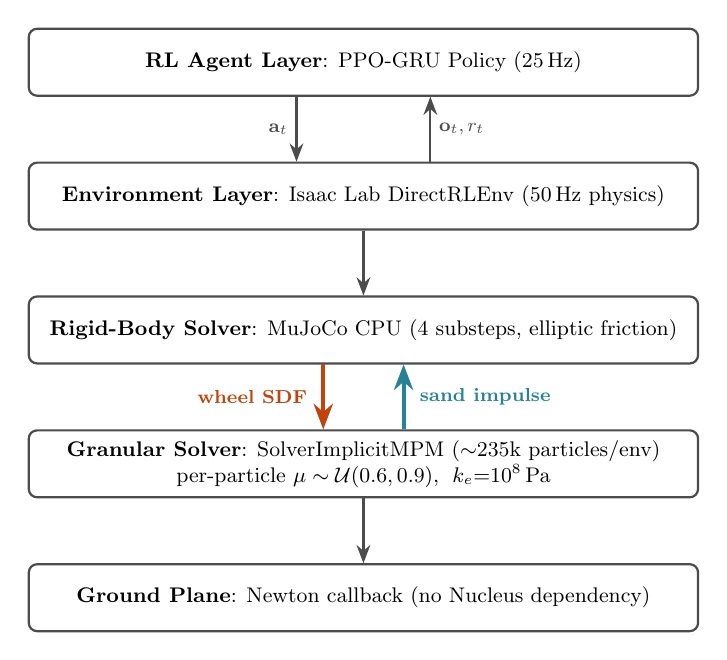
\begin{tikzpicture}[
      node distance=0.5cm,
      layer/.style={rectangle, draw=black!55, fill=white, thick, rounded corners=3pt,
                    minimum height=1.0cm, minimum width=10cm,
                    align=center, font=\small},
      arrow/.style={-Stealth, thick, color=black!70},
      scale=0.85, transform shape
    ]
      \node[layer, fill=white, draw=black!70] (rl) at (0, 8.0)
          {\textbf{RL Agent Layer}: PPO-GRU Policy (25\,Hz)};
      \node[layer, fill=white, draw=black!70] (env) at (0, 6.0)
          {\textbf{Environment Layer}: Isaac Lab DirectRLEnv (50\,Hz physics)};
      \node[layer, fill=white, draw=black!70] (rigid) at (0, 4.0)
          {\textbf{Rigid-Body Solver}: MuJoCo CPU (4 substeps, elliptic friction)};
      \node[layer, fill=white, draw=black!70] (mpm) at (0, 2.0)
          {\textbf{Granular Solver}: SolverImplicitMPM (${\sim}235\text{k}$ particles/env)\\
           per-particle $\mu \sim \mathcal{U}(0.6,0.9)$,\; $k_e{=}10^{8}$\,Pa};
      \node[layer, fill=white, draw=black!70] (ground) at (0, 0.0)
          {\textbf{Ground Plane}: Newton callback (no Nucleus dependency)};
      %% Two-way coupling annotations
      \draw[arrow, line width=1.4pt, color=MarsRust]
          ($(rigid.south)+(-0.6,0)$) -- ($(mpm.north)+(-0.6,0)$)
          node[midway, left=0.1cm, font=\footnotesize\bfseries, text=MarsRust]
              {wheel SDF};
      \draw[arrow, line width=1.4pt, color=softcyan]
          ($(mpm.north)+(0.6,0)$) -- ($(rigid.south)+(0.6,0)$)
          node[midway, right=0.1cm, font=\footnotesize\bfseries, text=softcyan]
              {sand impulse};
      %% RL--env flow
      \draw[arrow] ($(rl.south)+(-1.0,0)$) -- ($(env.north)+(-1.0,0)$)
          node[midway, left, font=\footnotesize] {$\mathbf{a}_t$};
      \draw[arrow] ($(env.north)+(1.0,0)$) -- ($(rl.south)+(1.0,0)$)
          node[midway, right, font=\footnotesize] {$\mathbf{o}_t,r_t$};
      \draw[arrow] (env.south)  -- (rigid.north);
      \draw[arrow] (mpm.south)  -- (ground.north);
    \end{tikzpicture}%
  }
  \caption{Physics simulation stack. Two-way coupling: the rust arrow shows
    wheel SDF geometry displacing sand particles via the Newton MPM
    \texttt{compute\_body\_forces} kernel; the cyan arrow shows the resulting
    particle impulses feeding back as external forces on the rover body
    (\texttt{subtract\_body\_force} kernel applied between every physics step,
    not every policy step --- a decimation-2 mismatch fixed in v9). 64
    environments run in parallel, each with ${\sim}235$\,k MPM particles in a
    $3.5\times3.5\times0.6$\,m sand bed under Martian gravity
    ($g{=}3.72\,\text{m/s}^2$). The 0.6\,m depth provides $>2{\times}$ wheel
    radius of compliant sand below the deepest wheel position at the maximum
    curriculum sinkage of 0.28\,m, removing the rigid-floor confound that
    previously enabled a bulldoze exploit at 0.30\,m depth. Per-environment
    domain randomisation of sand friction is implemented as a per-particle
    \texttt{wp.array} written into the implicit-MPM solver's
    \texttt{material\_parameters.friction} buffer; a scalar post-init
    assignment is silently overwritten at solver construction and was a
    near-invisible bug in earlier versions of the pipeline.}
  \label{fig:physics_stack}
\end{figure}

\paragraph{Why split rigid and granular solvers across two engines?}
A reasonable question is why we do not use Newton for both the articulated
rover and the granular bed, given that Newton ships its own rigid-body
pipeline (\texttt{mujoco\_warp}). The split is deliberate, not incidental, and
rests on three points. (i)~\emph{Solver maturity for passive-joint
articulations.} The AAU rocker-bogie has a passive differential and two
passive rocker pivots; MuJoCo's constraint solver has a decade of validation
on exactly this class of mechanism (it is the backbone of MuJoCo Menagerie's
quadruped/rover models and of DeepMind Control Suite). Newton's
\texttt{mujoco\_warp} backend is newer and at the time of writing carries
upstream version constraints that conflict with the
\texttt{warp-lang${\geq}1.13$} required by Newton's
\texttt{SolverImplicitMPM}; resolving this in-tree would mean pinning
two upstream projects against each other. (ii)~\emph{Single-responsibility
separation.} Granular contact is the dominant source of solver stiffness in
this problem; isolating it in Newton's implicit MPM (which is the reason we
chose Newton in the first place) and handing the comparatively cheap
articulated-rigid problem to the mature CPU solver gives a clean failure
boundary --- if a physics artefact appears we know which solver to inspect.
(iii)~\emph{Coupling is one-shot per substep regardless.} The two-way
coupling is implemented as Warp kernels that read wheel SDF poses and write
external body forces; the rigid-body engine on the other side of that
interface is interchangeable, so using MuJoCo CPU here loses no expressive
power that Newton's rigid pipeline would add. The architectural cost we pay is
that the rigid-body integrator is CPU-bound; in practice this is hidden by
the MPM solver, which saturates the GPU and is the actual wall-clock
bottleneck. The separation also has a useful side-effect for review: it
removes any implicit shared-state leakage between the rigid and granular
solvers, since the only information that crosses the engine boundary is the
SDF/impulse exchange that is explicit in
Figure~\ref{fig:physics_stack}.

\begin{figure}[!htbp]
  \centering
  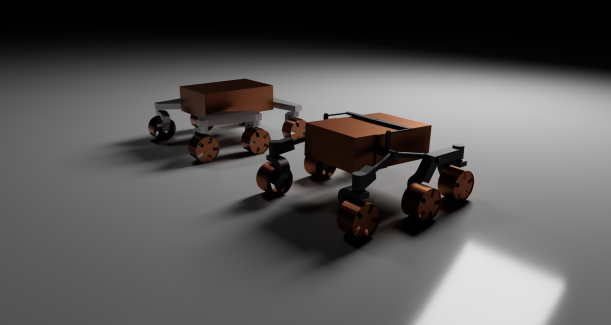
\includegraphics[width=0.49\linewidth]{rl_rover_lab_usd.png}\hfill
  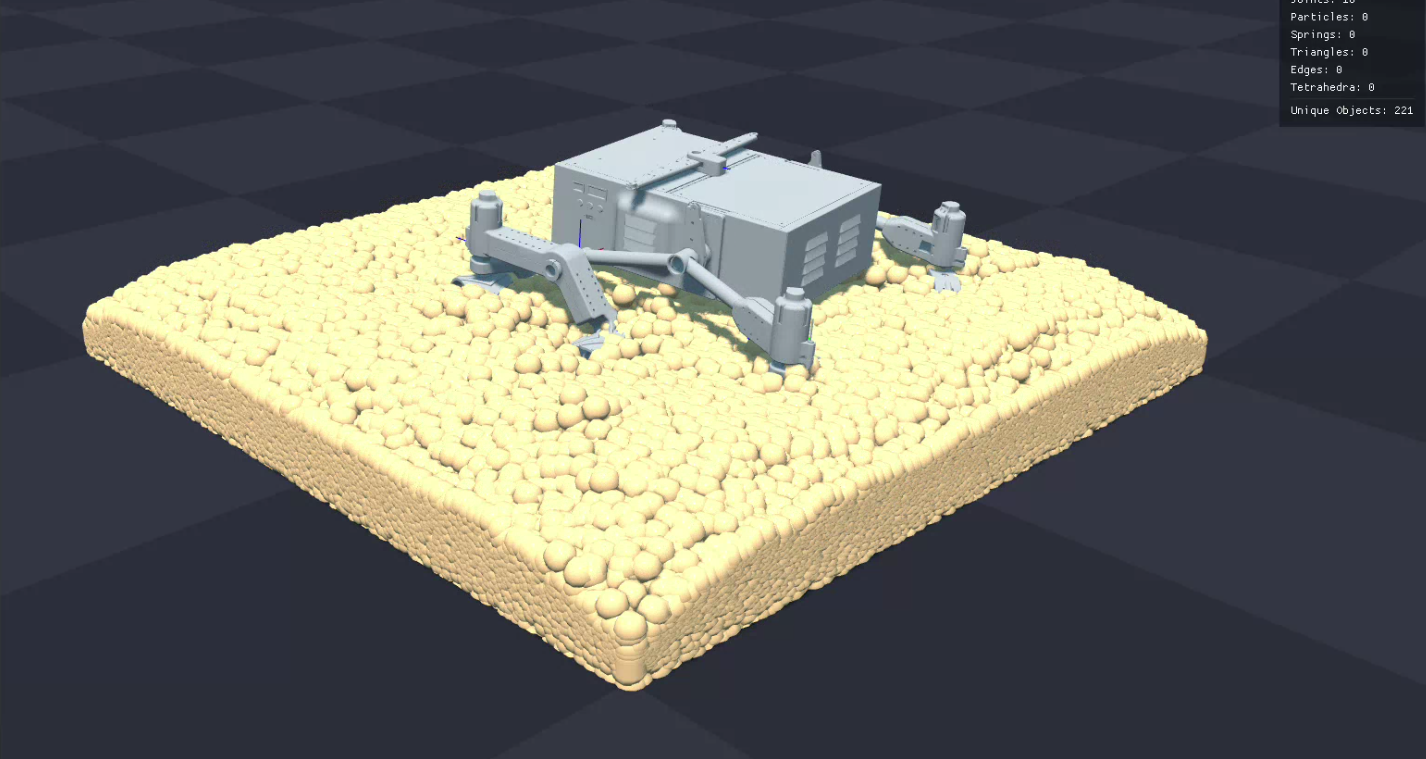
\includegraphics[width=0.49\linewidth]{paper_rover_entrapment.png}\\[3pt]
  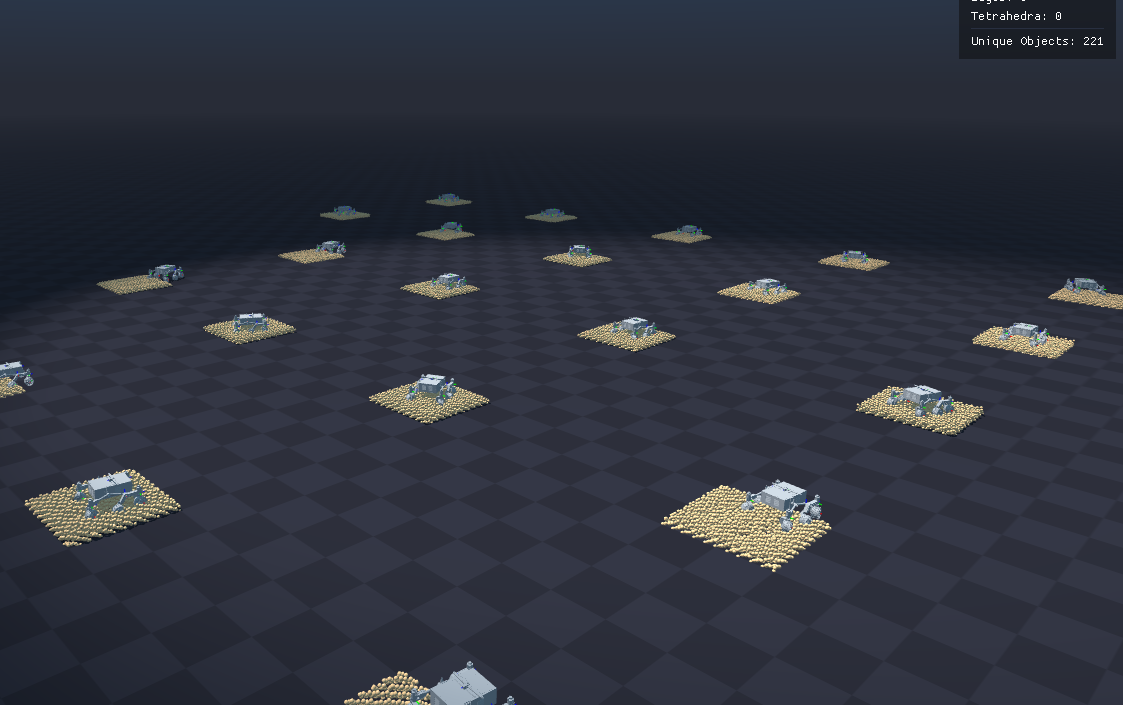
\includegraphics[width=0.49\linewidth]{parallel_training_multi_env.png}\hfill
  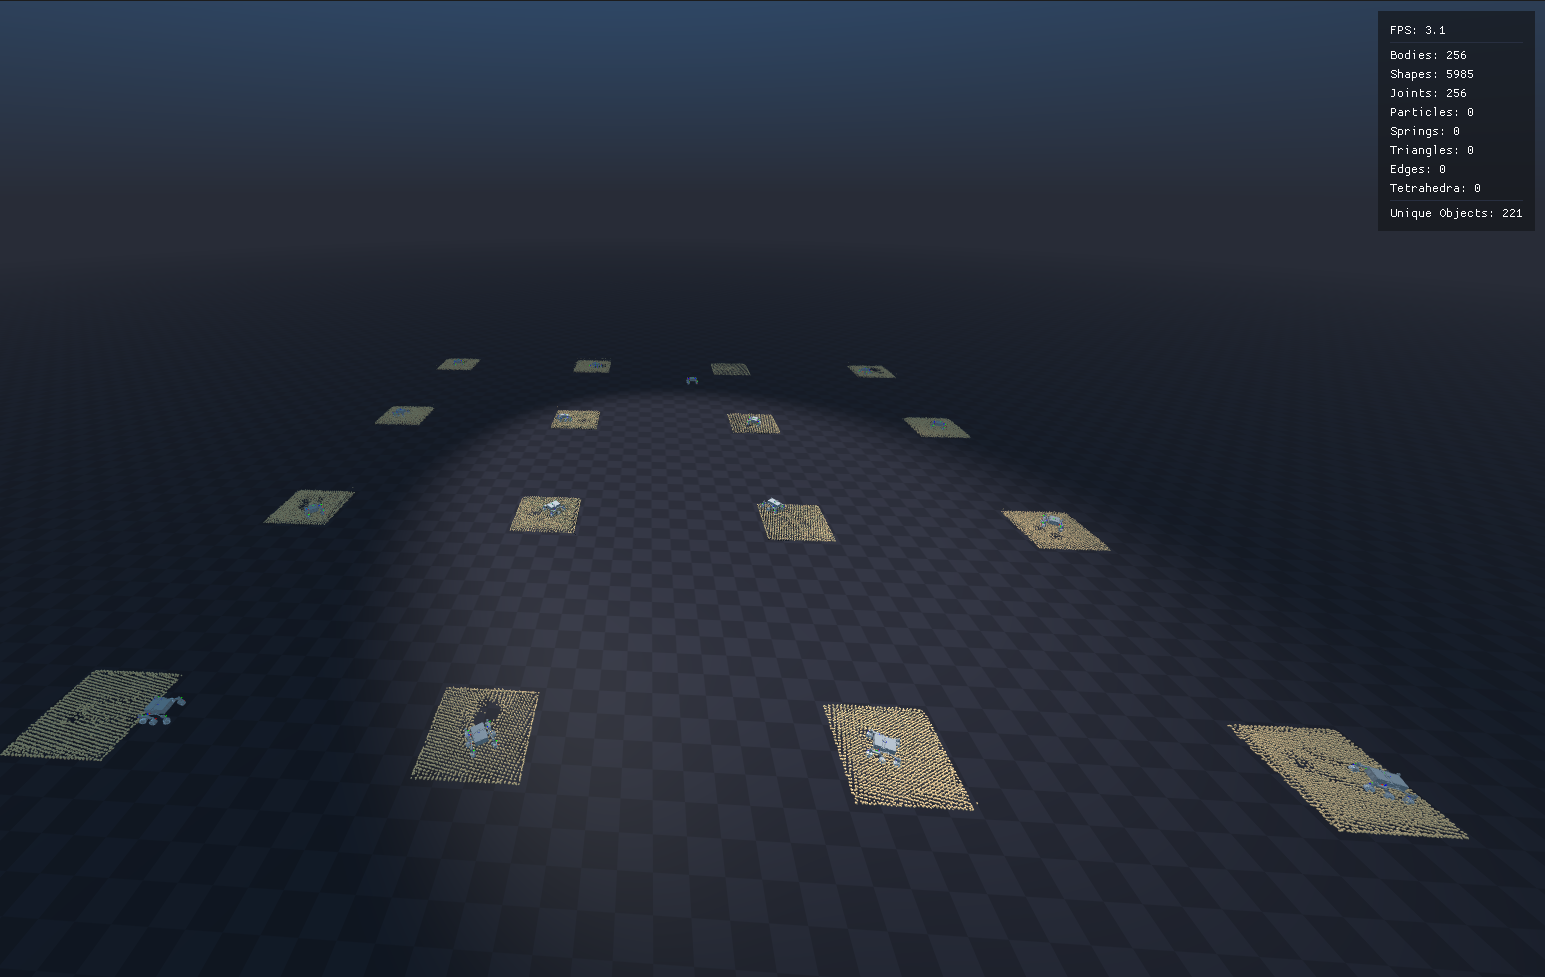
\includegraphics[width=0.49\linewidth]{parallel_training_multi_env2.png}
  \caption{Robot platform, entrapment scenario, and parallel training layout.
    The AAU 6-wheel rocker-bogie rover is loaded from the RLRoverLab USD asset
    and placed partially buried in the Newton MPM sand bed at the start of each
    recovery episode; displaced particles are visible around the contact
    patches. 16 cloned environments run in parallel on a single workstation,
    each with an independent ${\sim}235$\,k-particle sand bed under Martian
    gravity ($g{=}3.72\,\text{m/s}^2$).}
  \label{fig:rover_mpm}
\end{figure}

% ══════════════════════════════════════════════════════════════
%  FULL-WIDTH FIGURE: Per-wheel coupling  (two-column)
% ══════════════════════════════════════════════════════════════
\begin{figure*}[!htbp]
  \centering
  \resizebox{0.82\textwidth}{!}{%
    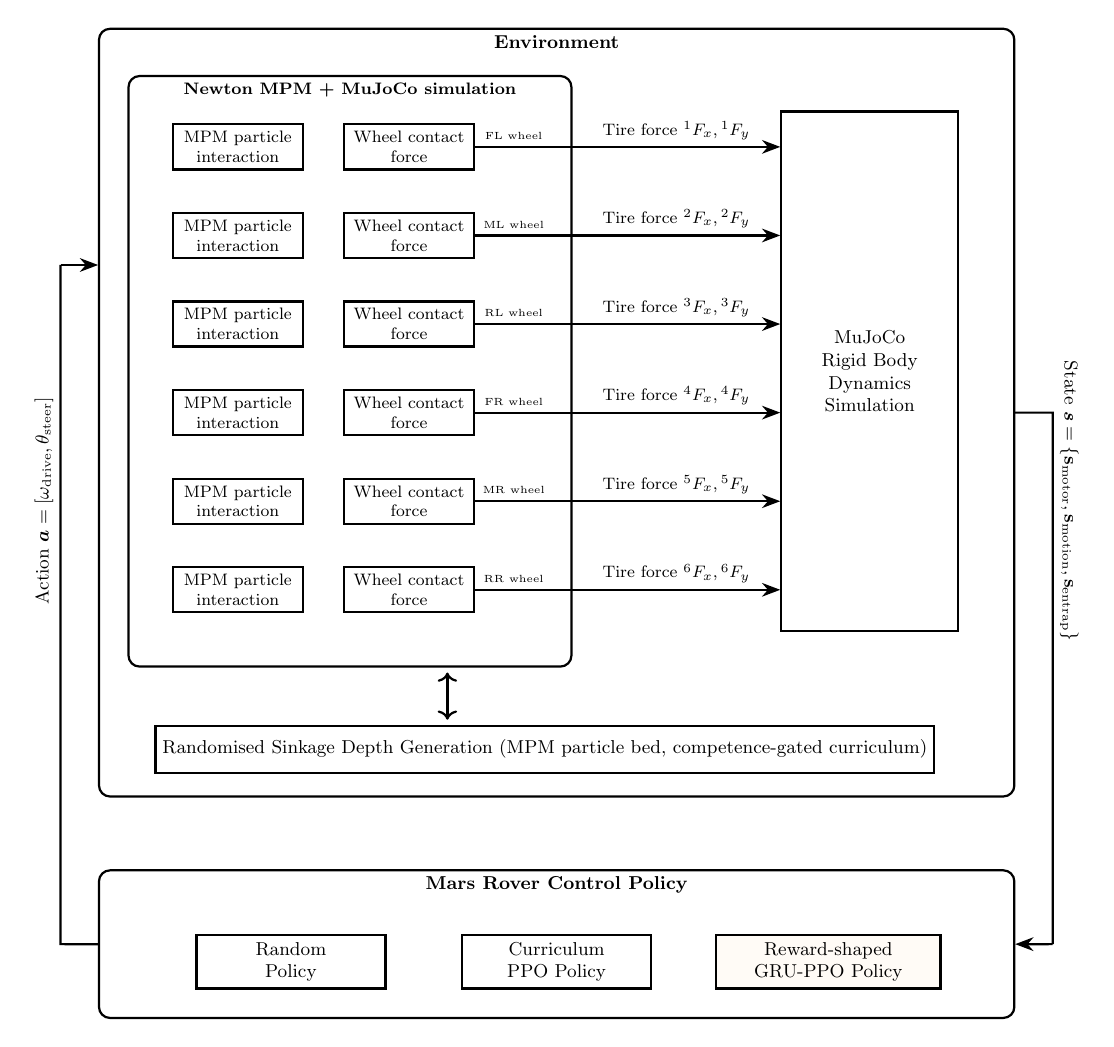
\begin{tikzpicture}[
      scale=0.75, transform shape,
      outerbox/.style={rectangle, draw=black, thick, rounded corners},
      innerbox/.style={rectangle, draw=black, thick, fill=lightblue!30,
                       minimum height=0.8cm, align=center, font=\small},
      wheelbox/.style={rectangle, draw=black, thick, fill=white,
                       minimum height=0.7cm, minimum width=2.2cm,
                       align=center, font=\footnotesize},
      arrow/.style={-Stealth, thick},
      every node/.style={font=\small}
    ]
      %% Outer Environment box
      \node[outerbox, fill=white, minimum width=15.5cm, minimum height=13cm,
            label={[font=\small\bfseries, anchor=north]north:Environment}]
            (envbox) at (0.2, 0.5) {};
      %% Inner Simulation box
      \node[outerbox, fill=white, minimum width=7.5cm, minimum height=10cm,
            label={[font=\footnotesize\bfseries, anchor=north]north:%
              Newton MPM + MuJoCo simulation}]
            (motorsim) at (-3.3, 1.2) {};
      %% Rigid body box
      \node[innerbox, minimum width=3cm, minimum height=8.8cm, fill=white]
            (rigidbody) at (5.5, 1.2)
            {MuJoCo\\Rigid Body\\Dynamics\\Simulation};
      %% 6-wheel rows
      \foreach \i/\name/\ypos in {1/FL/5, 2/ML/3.5, 3/RL/2,
                                    4/FR/0.5, 5/MR/-1, 6/RR/-2.5}{
        \node[wheelbox] (motor\i) at (-5.2, \ypos) {MPM particle\\interaction};
        \node[wheelbox] (tire\i)  at (-2.3, \ypos) {Wheel contact\\force};
        \coordinate (simright) at (motorsim.east|-tire\i.east);
        \draw[arrow] (tire\i.east) -- (rigidbody.west|-tire\i.east);
        \node[font=\tiny, anchor=south]
              at ($(tire\i.east)!0.4!(simright)$) {\name{} wheel};
        \node[font=\footnotesize, anchor=south]
              at ($(simright)!0.5!(rigidbody.west|-tire\i.east)$)
              {Tire force ${}^{\i}F_x,{}^{\i}F_y$};
      }
      %% Curriculum terrain
      \node[innerbox, minimum width=13cm, fill=white] (randterrain) at (0, -5.2)
            {Randomised Sinkage Depth Generation (MPM particle bed,
             competence-gated curriculum)};
      \coordinate (arrowpos) at ($(motorsim.south)!0.5!(randterrain.north)$);
      \draw[thick, <->] ($(arrowpos)+(0,-0.4)$) -- ($(arrowpos)+(0,0.4)$);
      %% Control policy box
      \node[outerbox, fill=white, minimum width=15.5cm, minimum height=2.5cm,
            label={[font=\small\bfseries, anchor=north]north:Mars Rover Control Policy}]
            (policybox) at (0.2, -8.5) {};
      \node[innerbox, fill=white, minimum width=3.2cm] (expert)   at (-4.3, -8.8)
            {Random\\Policy};
      \node[innerbox, fill=white, minimum width=3.2cm] (imitator) at ( 0.2, -8.8)
            {Curriculum\\PPO Policy};
      \node[innerbox, fill=lightorange!20, minimum width=3.8cm] (fusion) at (4.8, -8.8)
            {Reward-shaped\\GRU-PPO Policy};
      %% Action/state loops
      \draw[thick] (policybox.west) -- (-8.2, -8.5) -- (-8.2, 3);
      \draw[arrow] (-8.2, 3) -- (envbox.west|-{(-8.2,3)});
      \node[font=\small, rotate=90, anchor=south] at (-8.2, -1)
            {Action $\boldsymbol{a}=[\omega_\text{drive},\theta_\text{steer}]$};
      \draw[thick] (envbox.east) -- (8.6, 0.5) -- (8.6, -8.5);
      \draw[arrow] (8.6, -8.5) -- (policybox.east);
      \node[font=\small, rotate=-90, anchor=south] at (8.6, -1)
            {State $\boldsymbol{s}=\{\mathbf{s}_\text{motor},
             \mathbf{s}_\text{motion}, \mathbf{s}_\text{entrap}\}$};
    \end{tikzpicture}%
  }
  \caption{Simulation framework showing per-wheel coupling. Each of the six
    wheels produces MPM particle interaction forces and wheel contact forces, fed
    to the MuJoCo rigid-body solver as per-wheel tyre forces ${}^iF_x, {}^iF_y$.
    The control policy receives the full 29D observation and issues 10D actions
    (6 drive + 4 steer).}
  \label{fig:simulation_framework}
\end{figure*}

% ══════════════════════════════════════════════════════════════
\begin{figure*}[!htbp]
  \centering
  \hspace*{1.2cm}\resizebox{0.92\textwidth}{!}{%
    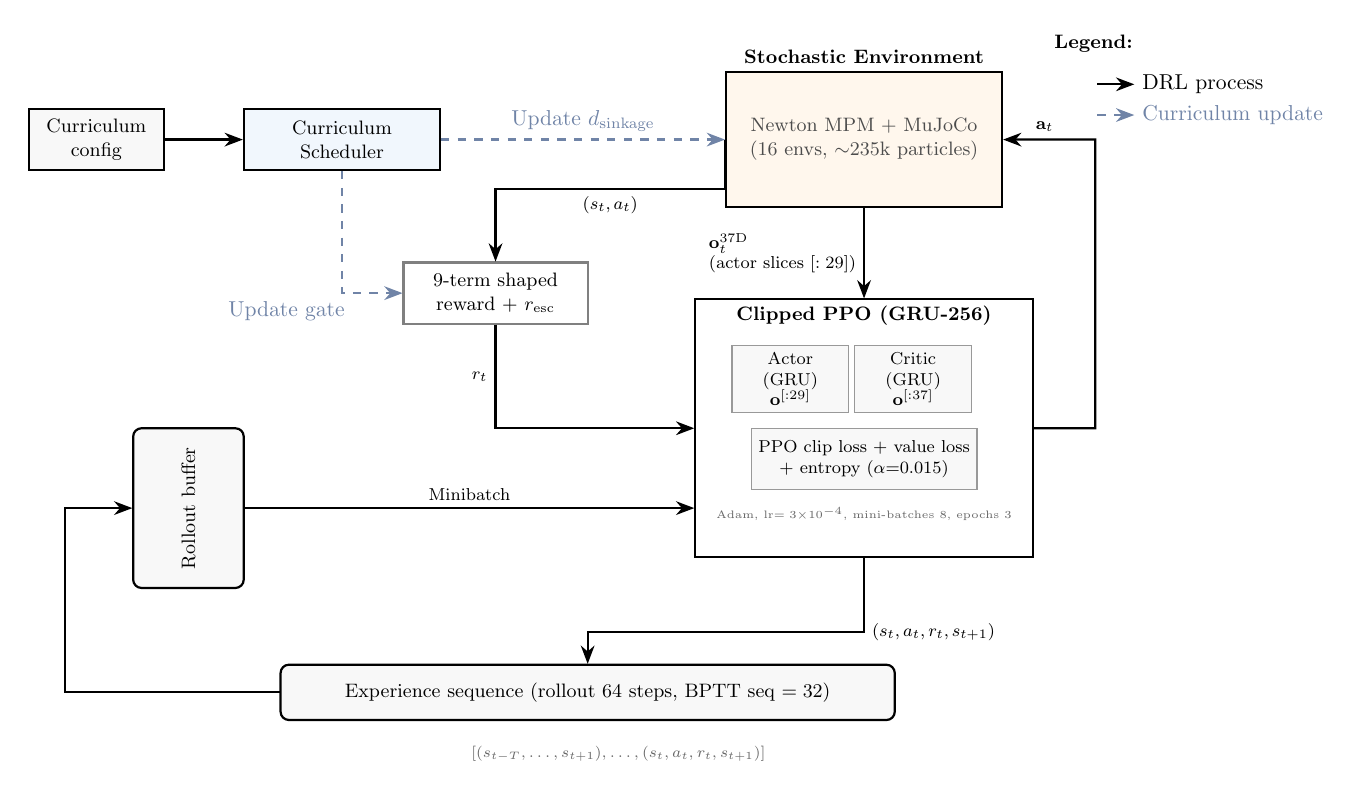
\begin{tikzpicture}[
      scale=0.78, transform shape,
      basebox/.style={rectangle, draw=black, thick, align=center, font=\small,
                      minimum height=1cm},
      scheduler/.style={basebox, fill=lightblue!40, minimum width=3.2cm},
      env/.style={basebox, fill=lightorange!40, minimum width=4.5cm,
                  minimum height=2.2cm},
      reward/.style={basebox, fill=white, minimum width=3cm, draw=black!50},
      ppo/.style={basebox, fill=white, minimum width=5.5cm, minimum height=4.2cm},
      replay/.style={basebox, fill=boxgray, minimum width=1.8cm,
                     minimum height=2.6cm, rounded corners=3pt},
      seq/.style={basebox, fill=boxgray, minimum width=10cm,
                  minimum height=0.9cm, rounded corners=3pt},
      inner/.style={rectangle, draw=black!40, fill=boxgray, align=center,
                    font=\footnotesize, minimum height=0.8cm},
      arrow/.style={-Stealth, thick},
      dashedblue/.style={-Stealth, thick, dashed, color=headerblue!70},
    ]
      \node[basebox, fill=boxgray, minimum width=2.2cm] (cfg) at (-8.5, 5.5)
            {Curriculum\\config};
      \node[scheduler] (sched) at (-4.5, 5.5) {Curriculum\\Scheduler};
      \draw[arrow] (cfg.east) -- (sched.west);
      \node[env] (env) at (4, 5.5) {};
      \node[font=\small\bfseries, anchor=south] at (env.north)
            {Stochastic Environment};
      \node[font=\small, text=black!70, align=center] at (4, 5.5)
            {Newton MPM + MuJoCo\\(16 envs, $\sim$235k particles)};
      \node[anchor=south east, font=\small\bfseries] at (8.5, 6.8) {Legend:};
      \draw[arrow] (7.8, 6.4) -- (8.4, 6.4) node[right] {DRL process};
      \draw[dashedblue] (7.8, 5.9) -- (8.4, 5.9)
            node[right] {Curriculum update};
      \node[reward] (reward) at (-2, 3) {9-term shaped\\reward + $r_\text{esc}$};
      \node[ppo] (ppo) at (4, 0.8) {};
      \node[font=\small\bfseries, anchor=north] at (ppo.north)
            {Clipped PPO (GRU-256)};
      \node[inner, minimum width=1.9cm] (act) at (2.8, 1.6)
            {Actor\\(GRU)\\$\mathbf{o}^{[:29]}$};
      \node[inner, minimum width=1.9cm] (crit) at (4.8, 1.6)
            {Critic\\(GRU)\\$\mathbf{o}^{[:37]}$};
      \node[inner, minimum width=3.6cm, minimum height=1cm] (loss) at (4, 0.3)
            {PPO clip loss + value loss\\+ entropy ($\alpha{=}0.015$)};
      \node[font=\tiny, text=black!60, anchor=north]
            at ($(loss.south)+(0,-0.15)$)
            {Adam, lr$=3{\times}10^{-4}$, mini-batches~8, epochs~3};
      \node[replay] (replay) at (-7, -0.5)
            {\rotatebox{90}{Rollout buffer}};
      \node[seq] (seq) at (-0.5, -3.5)
            {Experience sequence (rollout 64 steps, BPTT seq~$=32$)};
      \node[font=\scriptsize, text=black!60] at (0.0, -4.5)
            {$[(s_{t-T}, \dots, s_{t+1}), \dots, (s_t, a_t, r_t, s_{t+1})]$};
      \draw[dashedblue] (sched.east) -- (env.west |- sched.east)
            node[midway, above, text=headerblue!70] {Update $d_\text{sinkage}$};
      \draw[dashedblue] (sched.south) -- (sched.south |- reward.west) -- (reward.west)
            node[pos=0.3, below, xshift=-1.2cm, text=headerblue!70]
                {Update gate};
      \draw[arrow] (env.west) -- ++(0,-0.8) -| (reward.north)
            node[pos=0.25, below, font=\footnotesize] {$(s_t, a_t)$};
      \draw[arrow] (env.south) -- (ppo.north)
            node[midway, left, font=\footnotesize, align=left]
                 {$\mathbf{o}_t^{37\text{D}}$\\(actor slices $[:29]$)};
      \draw[arrow] (ppo.east) -- ++(1.0,0) coordinate(atmp)
            -- (atmp |- env.east) -- (env.east)
            node[pos=0.55, above, font=\footnotesize] {$\mathbf{a}_t$};
      \draw[arrow] (reward.south) |- (ppo.west)
            node[pos=0.25, left, font=\footnotesize] {$r_t$};
      \draw[arrow] (ppo.south) -- ++(0, -1.2) -| (seq.north)
            node[pos=0.0, right, font=\footnotesize] {$(s_t, a_t, r_t, s_{t+1})$};
      \draw[arrow] (seq.west) -- ++(-3.5, 0) |- (replay.west);
      \draw[arrow] (replay.east) -- (ppo.west |- replay.east)
            node[midway, above, font=\footnotesize] {Minibatch};
    \end{tikzpicture}%
  }
  \caption{DRL training loop: PPO-GRU with competence-gated curriculum scheduler
    and asymmetric actor--critic. The scheduler updates the sinkage depth
    $d_\text{sinkage}$ and the gate state based on rolling-window escape
    statistics. The stochastic environment (Newton MPM + MuJoCo, 16 parallel
    envs) emits a 37-dimensional observation tensor; the \emph{actor} consumes
    only the first 29 dimensions (proprioceptive features available at
    deployment), while the \emph{critic} consumes the full 37D tensor including
    8 privileged simulator-only features (true sinkage, wheel burial ratio,
    sand-force proxy, body linear velocity, yaw rate, chassis~$z$). This
    asymmetry yields lower-variance value estimates without leaking
    unobservable state into the policy, since only the actor's 29D head is
    exported for ONNX deployment. Shaped rewards drive the clipped surrogate
    loss; rollouts feed a buffer that supplies BPTT minibatches (sequence
    length~32).}
  \label{fig:training_loop}
\end{figure*}

\section{Methodology}
\label{sec:method}

\subsection{Robot Platform}

The \textit{AAU Mars Rover}~\cite{rlroverlab} is a 6-wheel rocker-bogie platform
(wheel radius $r{=}0.10$\,m) with 6 independent drive joints (velocity control,
$\pm6$\,rad/s, $\tau_{\max}{=}40$\,Nm), 4 steering joints (position control,
$\pm0.6$\,rad), and passive rocker-bogie differential joints. The simulation
couples the Newton physics engine~\cite{newton} with Isaac Lab~\cite{isaaclab}
and MuJoCo~\cite{todorov2012mujoco} as the rigid-body backend under Martian
gravity ($g{=}3.72\,\text{m/s}^2$, 62\% reduction from Earth).

The drive actuators use implicit torque control (stiffness~$=0$,
damping~$=4000$\,Ns/m, effort limit~$40$\,Nm). At free-driving steady state
($v_\text{err}{\approx}0.005$\,rad/s), $\tau{\approx}20$\,Nm (ratio~$\approx0.50$).
Under burial ($v_\text{err}{\approx}2$\,rad/s), the implicit-controller torque
$\tau \,{=}\, k_d v_\text{err} \,{=}\, 8000$\,Nm is clipped at the actuator
ceiling so $\tau\to40$\,Nm (ratio~$=1.0$). Crucially, the saturation arises
from \emph{velocity-error pinning} in the actuator dynamics, \emph{not} from a
bang-bang policy: the policy still modulates command velocity, but the realised
torque rails because the steady-state $v_\text{err}$ in deep sand exceeds the
$k_d$-weighted ceiling. An earlier iteration lowered the cap to 22\,Nm to
``ease saturation''; this misdiagnosis starved legitimate escape thrust and
drove mean forward velocity from 0.46 to 0.15\,m/s. The control surface that
actually shapes saturation behaviour is the slip-conditional grind penalty
$p_\text{grind}$ (Sec.~\ref{sec:reward}), not the effort cap.

\subsection{Granular Sand Simulation}
\label{sec:granular}

Each of the 16 parallel environments contains a $3.5{\times}3.5{\times}0.60$\,m
MPM sand bed (voxel size $0.05$\,m, PPC~$=2.0$, ${\sim}235\,000$ particles),
with friction $\mu \sim \mathcal{U}(0.6, 0.9)$ per environment per reset
(realised via a per-particle \texttt{wp.array} written into the implicit-MPM
solver's \texttt{material\_parameters.friction} buffer, since a scalar
post-init assignment is silently overwritten at solver construction) and bulk
modulus $k_e{=}10^{8}$\,Pa, the physical range for terrestrial dry sand
(${\sim}30$--$100$\,MPa). An earlier iteration used the Newton reference
value $k_e{=}10^{15}$\,Pa, which made the bed effectively incompressible:
wheel impulses bounced off a near-rigid floor, and the policy learned a
``hop-and-grab'' strategy that does not transfer to physical regolith.
Lowering $k_e$ to a physically realistic value is admissible because the
implicit MPM solver is unconditionally stable at any $k_e$. The bed depth
$0.60$\,m provides $>2{\times}$ wheel-radius of compliant sand below the
maximum curriculum sinkage (0.28\,m), eliminating the rigid-floor confound.
The square footprint, symmetric in all four cardinal directions, ensures
omnidirectional escape training is not biased by asymmetric runway length.

A 60-step ($1.2$\,s at $\Delta t{=}0.02$\,s per physics step) settlement
window after each reset clamps per-body sand forces to 250\,N and torques to
40\,Nm, allowing particles to relax around the wheels without launching the
chassis under the sudden SDF--particle overlap created by teleportation. The
window is intentionally generous: an earlier 20-step / 800\,N regime caused
${\approx}37\%$ of episodes to be flagged as ``trivial escapes'' driven by the
unrelaxed compression spike, corrupting the curriculum gate.

\subsection{Omnidirectional Escape and Zero-Shot Goal Generalisation}
\label{sec:omnidir}

Training with a fixed escape heading (e.g.~$+x$) produces a policy that can
only escape in that direction, failing when the entrapment zone lies across the
path to a GPS waypoint. Instead, at the start of each episode we sample:
\begin{equation}
  \phi_\text{esc} \sim \mathcal{U}(0, 2\pi)
\end{equation}
and orient the rover to face $\phi_\text{esc}$ (with $\pm5^\circ$ jitter).
The escape direction buffer $\hat{\mathbf{e}} = [\cos\phi_\text{esc},
\sin\phi_\text{esc}]^\top$ is used in the reward, not exposed in the observation.
The result is a \emph{heading-agnostic} policy that, in the body frame, always
``escapes forward.''

At deployment, the mode-switcher sets $\hat{\mathbf{e}}$ to the direction from the
current position toward GPS goal B:
\begin{equation}
  \hat{\mathbf{e}}_\text{deploy} =
  \frac{\mathbf{p}_B - \mathbf{p}_t}{\|\mathbf{p}_B - \mathbf{p}_t\|_2}
\end{equation}
This zero-shot goal-directed recovery requires no additional training or
fine-tuning: the heading generalisation learned over $\mathcal{U}(0,2\pi)$
episodes covers every GPS bearing.

\subsection{Reward Function}
\label{sec:reward}

\begin{equation}
  \begin{aligned}
  R_t &= r_{\text{prog}} + r_{\text{esc}} + r_{\text{esc,shaped}}
        + r_{\text{rock}} \\
      &\quad - p_{\text{slip}} - p_{\text{tilt}}
        - p_{\text{smooth}} - p_{\text{abn}}
        - p_{\text{rev}} - p_{\text{hop}} - p_{\text{grind}}
  \end{aligned}
  \label{eq:reward}
\end{equation}

\begin{table}[!htbp]
  \centering
  \caption{Shaped reward ($\Delta t{=}0.04$\,s). All terms multiply by $\Delta t$;
    the milestone bonus (weight~20) dominates during entrapment. Unlike
    Bi~\&~Ding~\cite{bi2026escape}, who use GAIL-fused rewards requiring expert
    demonstrations, every term here is hand-engineered from first principles and
    all progress terms are projected onto the \emph{world-frame} escape heading
    $\hat{\mathbf{e}}$ to prevent the body-frame reward-farming failure mode
    described in Sec.~\ref{sec:method}.}
  \label{tab:reward}
  \renewcommand{\arraystretch}{1.25}
  \begin{tabular}{@{}lcp{4.0cm}@{}}
    \toprule
    \textbf{Term} & \textbf{Wt.} & \textbf{Formula / Justification} \\
    \midrule
    $r_{\text{prog}}$
      & $+1.5$
      & $(\mathbf{v}_{xy} \cdot \hat{\mathbf{e}})\,\Delta t$ --- world-frame
        progress along $\hat{\mathbf{e}}$; \emph{unconditionally active}
        (never gated by $f_{\text{ent}}$) \\[2pt]
    $r_{\text{esc}}$
      & $+20$
      & Milestone bonuses at 0.5, 1.0, 2.0, 3.0\,m
        (scaled $0.1$/$0.2$/$0.4$/$1.0$) \\[2pt]
    $r_{\text{esc,shaped}}$
      & $+5$
      & $\Delta d_{\hat{\mathbf{e}}} \,\Delta t$ --- dense distance signal between
        milestones \\[2pt]
    $r_{\text{rock}}$
      & $+0.5$
      & $|\Delta (\mathbf{v}_{xy}\!\cdot\!\hat{\mathbf{e}})| \cdot f_\text{ent}\,
         \Delta t$ --- small bootstrap nudge for rocking while trapped \\[2pt]
    $p_{\text{slip}}$
      & $-0.5$
      & $\bar{\sigma}(1{-}f_\text{ent})\,\Delta t$ --- penalises spinning wheels
        only during free driving \\[2pt]
    $p_{\text{tilt}}$
      & $-0.3$
      & $\|\boldsymbol{\omega}_{xy}\|_2\,\Delta t$ --- stabilises body attitude
        \\[2pt]
    $p_{\text{smooth}}$
      & $-0.12$
      & $\|\mathbf{a}_t {-} \mathbf{a}_{t-1}\|_2\,\Delta t$ --- suppresses
        high-frequency jitter (raised from $0.05$ once
        $p_{\text{grind}}$ stopped relying on it as a saturation proxy) \\[2pt]
    $p_{\text{abn}}$
      & $-0.3$
      & $(-v_x)^+\! f_\text{anom}(1{-}f_\text{ent})\,\Delta t$ --- penalises
        reversing under slip anomaly \\[2pt]
    $p_{\text{rev}}$
      & $-1.0$
      & $\bigl(\!-\!\mathbf{v}_{xy}\!\cdot\!\hat{\mathbf{e}}\bigr)^+\!\Delta t$ ---
        symmetry-breaker: kills the backward-drift local optimum observed in
        early runs \\[2pt]
    $p_{\text{hop}}$
      & $-0.5$
      & $|v_z^\text{world}|\bigl(1{-}f_\text{grace}\bigr)\,\Delta t$ ---
        direct vertical-bounce penalty, gated by the burial-grace window so
        post-reset settle drift is not punished. Replaces the indirect
        $k_e{=}10^{15}$ rigid-floor signal that previously drove a
        ``hop-and-grab'' degenerate strategy \\[2pt]
    $p_{\text{grind}}$
      & $-0.30$
      & $\mathbf{1}[\bar{\sigma}{>}0.70]\,\|\mathbf{a}_t^{\text{drive}}\|_2\,\Delta t$
        --- slip-conditional command-magnitude penalty. Fires \emph{only}
        when wheels are actually slipping, providing the missing pressure
        against velocity-error pinning. Replaces an earlier
        $p_{\text{action-mag}}$ term that taxed all commands unconditionally
        and so could not break the saturation regime (the cap is
        $v_\text{err}$-set, not command-set) \\
    \bottomrule
  \end{tabular}
\end{table}

\textbf{Design rationale.}
The milestone bonus (weight~20) is sized so a single successful 3.0\,m escape
dominates an entire episode of shaping reward, making entrapment recovery the
sole primary objective. We initially set $r_\text{rock}$ weight to~5.0; this
produced a \emph{degenerate local optimum} in which the policy learned to farm
the rocking term by wheel-spinning in place with $v_x \approx 0$ and body-frame
oscillation. Two fixes were required: (i)~reduce the weight to~0.5 so rocking
only bootstraps progress, and (ii)~project all velocity-dependent reward terms
onto the world-frame escape heading $\hat{\mathbf{e}}$ rather than body-frame
$v_x$, eliminating yaw-wobble exploits. A separate symmetry-breaking term
$p_\text{rev}$ was necessary because, without it, a drift-backwards policy was
indistinguishable from a drift-forwards policy under the yaw-projected
shaping. The slip penalty is gated by $(1{-}f_\text{ent})$ so the agent is not
punished for the unavoidable slip of an already-trapped wheel; crucially
$r_\text{prog}$ is \emph{not} gated, so the policy continues to feel a
progress gradient throughout the entrapment phase.

\subsection{Slip-Anomaly Detection}
\label{sec:torque_anomaly}

The implicit-controller torque ratio
($\bar{\tau}{=}\tfrac{1}{6}\sum_i|\tau_i|/\tau_{\max}$) is an attractive but
ultimately uninformative anomaly signal: under burial, $v_\text{err}$ pins
the realised torque to the actuator ceiling regardless of policy command,
so $\bar{\tau}{\to}1.0$ throughout the entrapment phase, saturating any
threshold-based detector. We instead deploy a \emph{slip-anomaly} flag
$f_{\text{anom}}$ defined directly on the kinematic discrepancy between
commanded wheel speed and realised body motion:
\begin{equation}
  \begin{aligned}
    f_\text{anom} = 1 \;\iff\; &
      \Bigl( \bar{\sigma} > 0.92 \;\;\text{AND}\;\; |v_x| < 0.20\,\text{m/s} \Bigr) \\
      &\;\;\text{for} \geq 15\;\text{consecutive steps}
  \end{aligned}
  \label{eq:anomaly}
\end{equation}
where $\bar{\sigma}$ is the mean wheel slip ratio (Eq.~\eqref{eq:entrapment}).
Unlike the torque-ratio detector, the slip-anomaly flag is non-saturated under
both free driving (slip ${\approx}0.05$) and burial (slip ${\approx}0.85$ at
nominal sand, climbing past 0.92 only when the policy commands large wheel
speeds against an immobile chassis). The 0.92 threshold sits above the
typical burial baseline (0.85), so the flag fires specifically on the
``commanded-thrust-without-progress'' failure mode that the
$p_\text{grind}$ reward term penalises. Empirically the slip-anomaly fires
${\approx}0.6$\,s ahead of the slower 15-step entrapment counter
$f_\text{ent}$, providing the early-warning channel exploited by the
shaped reward.

\begin{figure}[!htbp]
  \centering
  
\includegraphics[width=\linewidth]{detection_flags.png}
  \caption{Dual-mode detector traces over training. The slip-ratio counter
    ($f_\text{ent}$) and torque-anomaly flag ($f_\text{anom}$) both fire during
    burial windows; the anomaly flag leads the slower entrapment counter,
    providing the early-warning signal exploited by the reward shaping.}
  \label{fig:detection_flags}
\end{figure}

\subsection{Competence-Gated Curriculum}

Sinkage depth is sampled each episode from a progressively deepening window:
\begin{equation}
  d \sim \mathcal{U}[d_{\min} + (d_{\max}-d_{\min})\cdot p,\; d_{\max}]
\end{equation}
with $d_{\min}{=}15$\,cm, $d_{\max}{=}28$\,cm (axle-level burial). Curriculum
progress $p \in [0,1]$ advances by $\Delta p{=}0.01$ per rollout only when two
conditions hold simultaneously over a 50-episode rolling window:
(i)~\emph{recent escape rate} $\geq 0.50$, and
(ii)~\emph{trivial-escape fraction} $< 0.25$ (episodes finishing in under 5\,s).
Both predicates must be satisfied: the first ensures the policy is competent at
the current level, the second prevents bounce-exploit policies (which escape by
physics artefact rather than learned behaviour) from advancing the curriculum.
The gate defaults \emph{fail-closed} until the rolling window is filled; an
earlier iteration used fail-open default which advanced the curriculum
prematurely on a mostly-empty window and caused the policy to stall at
$p{\approx}0.08$ with zero escape rate.

\begin{figure}[!htbp]
  \centering
  
\includegraphics[width=\linewidth]{curriculum_milestones.png}
  \caption{Competence-gated curriculum progress over training. Sinkage depth
    advances only when the policy sustains $\geq 0.50$ recent escape rate
    \emph{and} $<0.25$ trivial-escape fraction over a 50-episode window;
    visible plateaus correspond to the gate holding the policy at the current
    sinkage level until both predicates clear.}
  \label{fig:curriculum_milestones}
\end{figure}

\subsection{PPO Hyperparameters}

Rollout length 64 steps; BPTT sequence length 32; mini-batches 8; learning
epochs 3; learning rate $3{\times}10^{-4}$; clip $\epsilon{=}0.2$; discount
$\gamma{=}0.99$; GAE $\lambda{=}0.95$~\cite{schulman2015gae}; entropy coefficient
$\alpha{=}0.015$. An earlier configuration used $\alpha{=}0.03$, but with a
10-D continuous action space the per-step entropy bonus is
$\mathcal{O}(d_a)$, giving ${\approx}0.42$ per step under the initial
$\sigma{\approx}1$ policy --- comparable to the entire shaped reward magnitude
($0.1$--$0.3$ per step) early in training and so drowning the reward signal.
Halving $\alpha$ restores the reward gradient while still preventing collapse
(the policy std plateaus at ${\approx}1.05$ at convergence,
Fig.~\ref{fig:policy_metrics}). The policy is trained with PPO~\cite{schulman2017ppo}
via the skrl library~\cite{skrl}. Mini-batches~8 and epochs~3 (reduced from
the commonly used~5) prevent value-network overfit on easy early-curriculum
episodes while preserving gradient diversity across rollouts.

% ══════════════════════════════════════════════════════════════
%  FULL-WIDTH FIGURE: GRU-PPO Policy Architecture (two-column)
% ══════════════════════════════════════════════════════════════
\begin{figure*}[!htbp]
  \centering
  \resizebox{\textwidth}{!}{%
    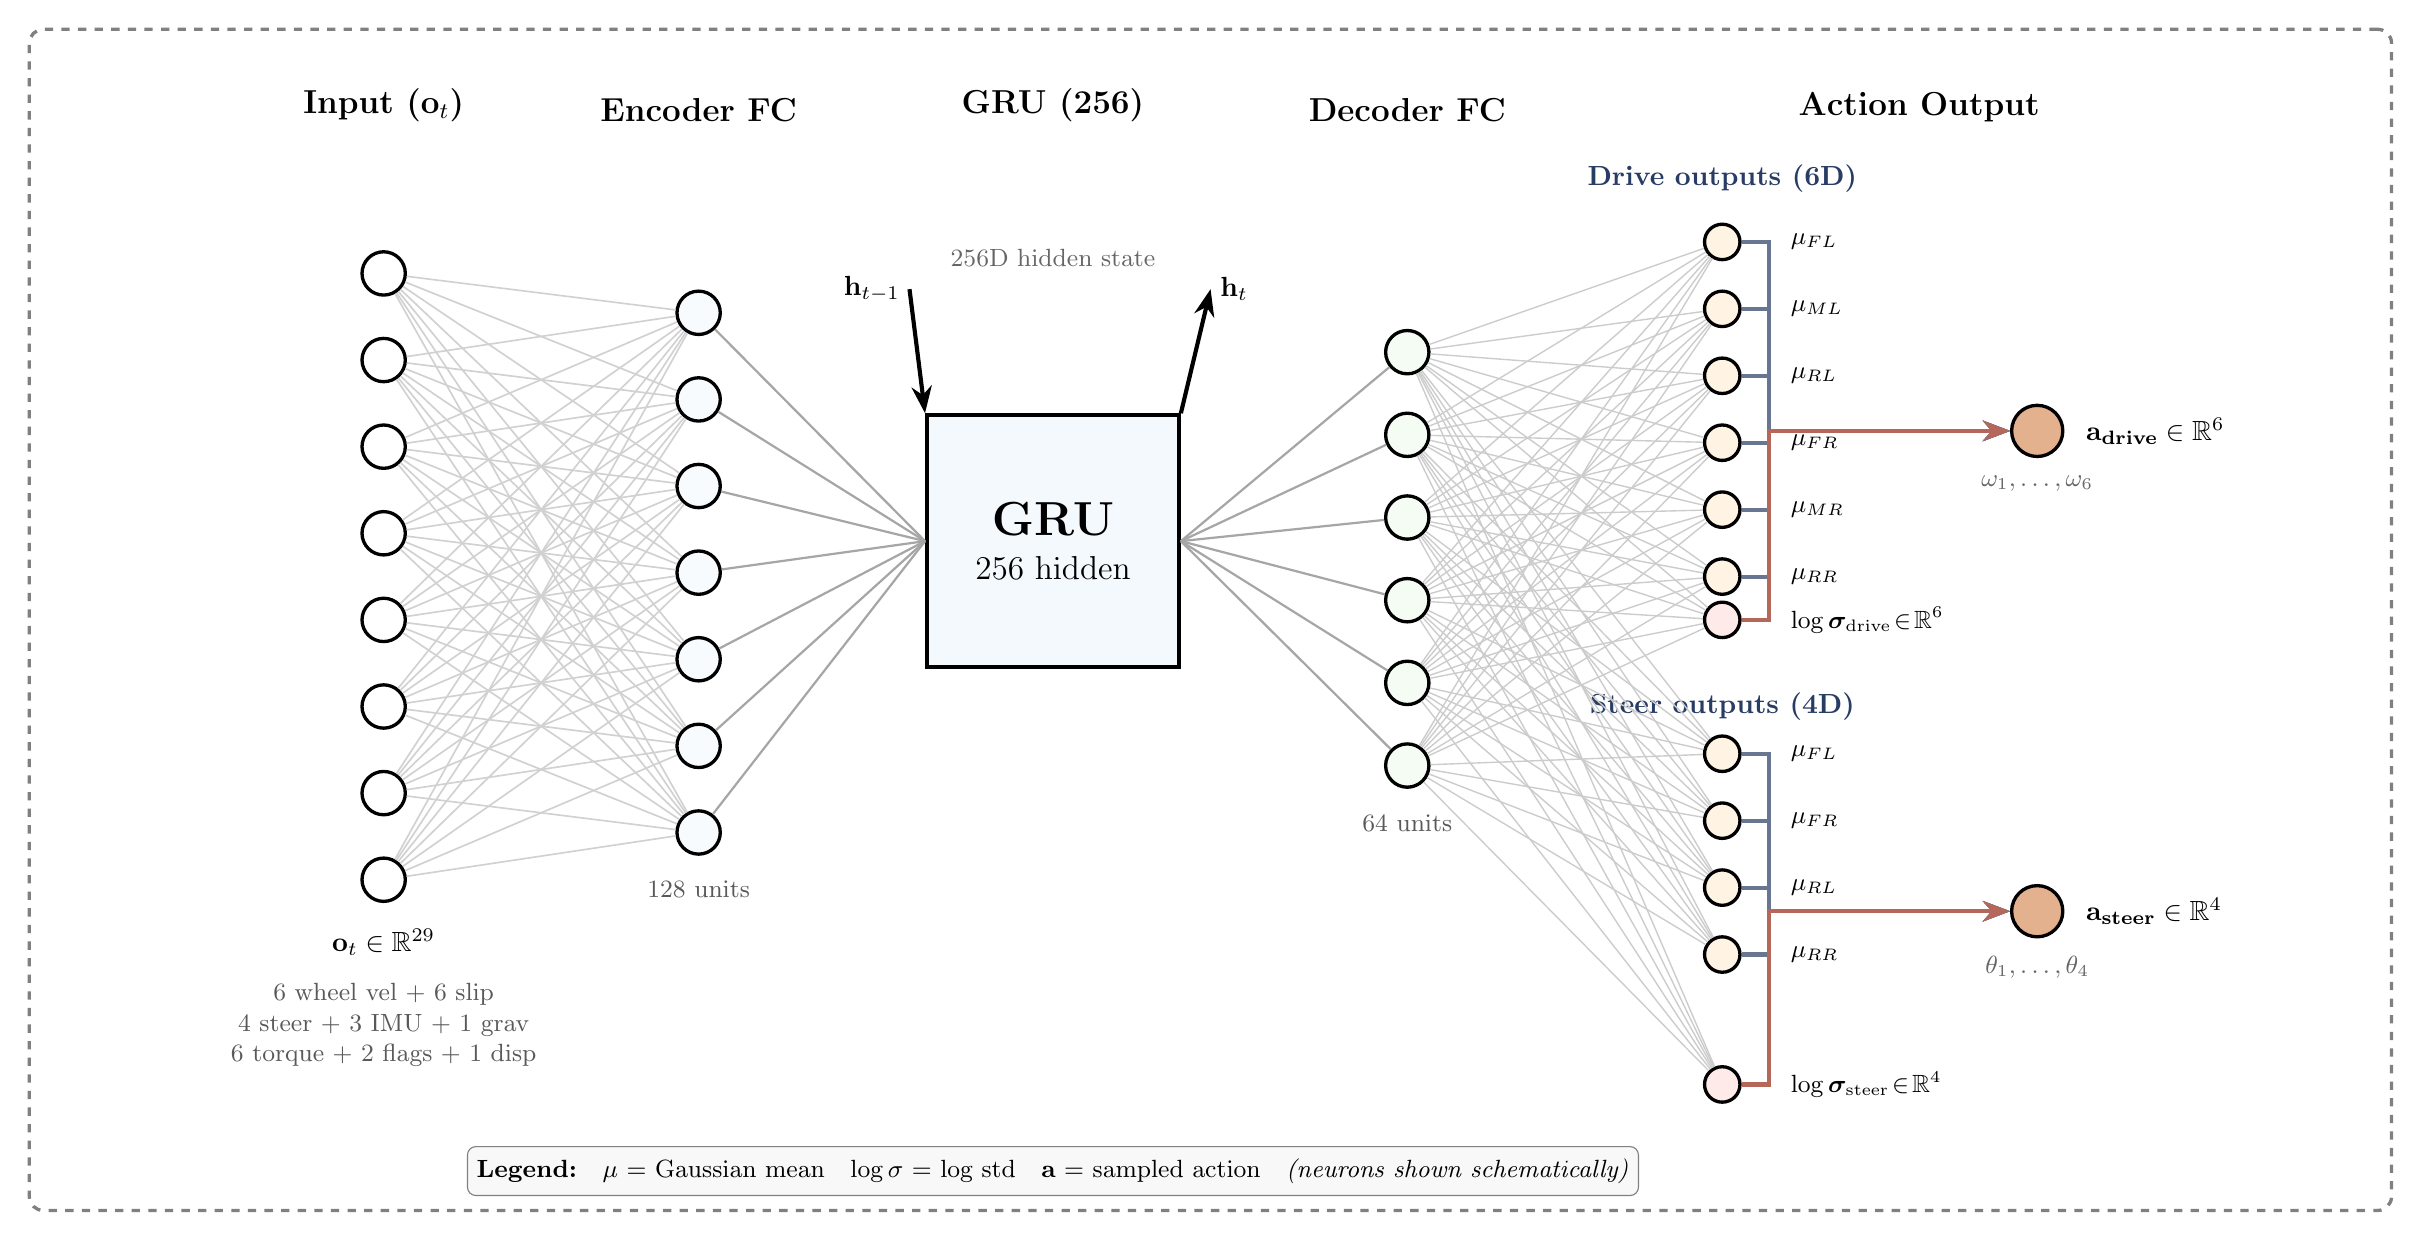
\begin{tikzpicture}[
      neuron/.style={circle, draw=black, line width=1.2pt,
                     minimum size=0.55cm, fill=white},
      grubox/.style={rectangle, draw=black, line width=1.4pt,
                     fill=lightblue!30, minimum width=3.2cm,
                     minimum height=3.2cm, align=center},
      arrow/.style={-Stealth, line width=1.5pt},
      dashedbox/.style={rectangle, draw=black!50, dashed,
                        line width=1.2pt, rounded corners=5pt},
    ]
      \node[dashedbox, minimum width=30cm, minimum height=15cm, fill=white]
            at (11.5, 0) {};
      %% Column headers
      \node[font=\large\bfseries, anchor=south] at ( 1.0, 6.2) {Input ($\mathbf{o}_t$)};
      \node[font=\large\bfseries, anchor=south] at ( 5.0, 6.2) {Encoder FC};
      \node[font=\large\bfseries, anchor=south] at ( 9.5, 6.2) {GRU (256)};
      \node[font=\large\bfseries, anchor=south] at (14.0, 6.2) {Decoder FC};
      \node[font=\large\bfseries, anchor=south] at (20.5, 6.2) {Action Output};
      %% Input neurons (8 representative for 29D)
      \foreach \i in {1,...,8}{
        \pgfmathsetmacro{\ypos}{4.4 - (\i-1)*1.1}
        \node[neuron] (in\i) at (1.0, \ypos) {};
      }
      \node[font=\normalsize\bfseries, below=0.2cm of in8]
            {$\mathbf{o}_t \in \mathbb{R}^{29}$};
      \node[font=\small, text=black!65, align=center, below=0.9cm of in8]{
        6 wheel vel $+$ 6 slip\\
        4 steer $+$ 3 IMU $+$ 1 grav\\
        6 torque $+$ 2 flags $+$ 1 disp};
      %% FC encoder (128 units)
      \foreach \i in {1,...,7}{
        \pgfmathsetmacro{\ypos}{3.9 - (\i-1)*1.1}
        \node[neuron, fill=lightblue!20] (fc1\i) at (5.0, \ypos) {};
      }
      \node[font=\small, text=black!65, below=0.2cm of fc17] {128 units};
      \foreach \i in {1,...,8}{
        \foreach \j in {1,...,7}{
          \draw[black!18, line width=0.6pt] (in\i) -- (fc1\j);
        }
      }
      %% GRU cell
      \node[grubox] (gru) at (9.5, 1.0) {\textbf{\LARGE GRU}\\[4pt]\large 256 hidden};
      \node[font=\normalsize\itshape] (ht_in)  at (7.2, 4.2) {$\mathbf{h}_{t-1}$};
      \node[font=\normalsize\itshape] (ht_out) at (11.8, 4.2) {$\mathbf{h}_{t}$};
      \draw[arrow] (ht_in.east)    -- (gru.north west);
      \draw[arrow] (gru.north east) -- (ht_out.west);
      \node[font=\small, text=black!60] at (9.5, 4.6) {256D hidden state};
      \foreach \i in {1,...,7}{
        \draw[black!35, line width=0.8pt] (fc1\i) -- (gru.west);
      }
      %% FC decoder (64 units)
      \foreach \i in {1,...,6}{
        \pgfmathsetmacro{\ypos}{3.4 - (\i-1)*1.05}
        \node[neuron, fill=lightgreen!30] (fc2\i) at (14.0, \ypos) {};
      }
      \node[font=\small, text=black!65, below=0.2cm of fc26] {64 units};
      \foreach \i in {1,...,6}{
        \draw[black!35, line width=0.8pt] (gru.east) -- (fc2\i);
      }
      %% Drive output head (6D)
      \node[font=\normalsize\bfseries, text=deepblue] at (18.0, 5.6)
            {Drive outputs (6D)};
      \foreach \i/\name in {1/FL, 2/ML, 3/RL, 4/FR, 5/MR, 6/RR}{
        \pgfmathsetmacro{\ypos}{4.8 - (\i-1)*0.85}
        \node[neuron, fill=lightorange!60, minimum size=0.45cm] (mu_d\i)
              at (18.0, \ypos) {};
        \node[font=\small, right=0.5cm of mu_d\i] {$\mu_{\name}$};
      }
      \node[neuron, fill=lightred!60, minimum size=0.45cm] (ls_d)
            at (18.0, 0.0) {};
      \node[font=\small, right=0.5cm of ls_d]
           {$\log\boldsymbol{\sigma}_{\text{drive}}\!\in\!\mathbb{R}^{6}$};
      %% Steer output head (4D)
      \node[font=\normalsize\bfseries, text=deepblue] at (18.0, -1.1)
            {Steer outputs (4D)};
      \foreach \i/\name in {1/FL, 2/FR, 3/RL, 4/RR}{
        \pgfmathsetmacro{\ypos}{-1.7 - (\i-1)*0.85}
        \node[neuron, fill=lightorange!60, minimum size=0.45cm] (mu_s\i)
              at (18.0, \ypos) {};
        \node[font=\small, right=0.5cm of mu_s\i] {$\mu_{\name}$};
      }
      \node[neuron, fill=lightred!60, minimum size=0.45cm] (ls_s)
            at (18.0, -5.9) {};
      \node[font=\small, right=0.5cm of ls_s]
           {$\log\boldsymbol{\sigma}_{\text{steer}}\!\in\!\mathbb{R}^{4}$};
      %% Sampled actions
      \node[neuron, fill=accentorange!50, minimum size=0.65cm]
            (a_d) at (22.0,  2.4) {};
      \node[font=\normalsize\bfseries, right=0.15cm of a_d]
            {$\mathbf{a}_{\text{drive}} \in \mathbb{R}^6$};
      \node[font=\small, text=black!60, below=0.1cm of a_d]
            {$\omega_1,\ldots,\omega_6$};
      \node[neuron, fill=accentorange!50, minimum size=0.65cm]
            (a_s) at (22.0, -3.7) {};
      \node[font=\normalsize\bfseries, right=0.15cm of a_s]
            {$\mathbf{a}_{\text{steer}} \in \mathbb{R}^4$};
      \node[font=\small, text=black!60, below=0.1cm of a_s]
            {$\theta_1,\ldots,\theta_4$};
      %% FC2 → output head connections
      \foreach \i in {1,...,6}{
        \foreach \j in {1,...,6}{ \draw[black!20, line width=0.5pt] (fc2\i) -- (mu_d\j); }
        \foreach \j in {1,...,4}{ \draw[black!20, line width=0.5pt] (fc2\i) -- (mu_s\j); }
        \draw[black!20, line width=0.5pt] (fc2\i) -- (ls_d);
        \draw[black!20, line width=0.5pt] (fc2\i) -- (ls_s);
      }
      %% Output → action arrows
      \foreach \i in {1,...,6}{
        \draw[arrow, color=deepblue!70] (mu_d\i.east) -- ++(0.35,0) |- (a_d.west);
      }
      \draw[arrow, color=marsred!70] (ls_d.east) -- ++(0.35,0) |- (a_d.west);
      \foreach \i in {1,...,4}{
        \draw[arrow, color=deepblue!70] (mu_s\i.east) -- ++(0.35,0) |- (a_s.west);
      }
      \draw[arrow, color=marsred!70] (ls_s.east) -- ++(0.35,0) |- (a_s.west);
      %% Legend
      \node[draw=black!50, fill=boxgray, rounded corners=3pt,
            align=left, font=\small] at (9.5, -7.0) {%
        \begin{tabular}{@{}l@{}}
          \textbf{Legend:}\quad
          $\mu$ = Gaussian mean\quad
          $\log\sigma$ = log std\quad
          $\mathbf{a}$ = sampled action\quad
          \textit{(neurons shown schematically)}
        \end{tabular}};
    \end{tikzpicture}%
  }
  \caption{GRU-PPO recurrent actor network. The 29D proprioceptive observation is
    encoded by a 128-unit fully connected layer, passed through a 256-unit GRU that
    maintains entrapment history $\mathbf{h}_t$, then decoded by a 64-unit FC layer
    that emits 10 means $\boldsymbol{\mu}_t \in \mathbb{R}^{10}$ (6D drive
    velocities $\|$ 4D steer angles). The log-standard-deviation
    $\log\boldsymbol{\sigma} \in \mathbb{R}^{10}$ is a state-independent
    learnable parameter vector (one per action dimension), following standard
    skrl \texttt{GaussianMixin} convention; the schematic shows it as a
    separate node since it is not a function of $\mathbf{o}_t$. The
    asymmetric critic has an identical recurrent backbone but reads the full
    37D observation (policy obs~$||$~8 privileged features) and outputs a
    scalar value $V_\phi(\mathbf{o}_t^{\text{full}}, \mathbf{h}_t)$. Only the
    actor's 29D slice is exported to ONNX for deployment, and the
    log-$\boldsymbol{\sigma}$ parameter is collapsed to its expectation
    $\boldsymbol{\mu}_t$ at inference time.}
  \label{fig:policy_arch}
\end{figure*}

% ══════════════════════════════════════════════════════════════
\section{Algorithms}
\label{sec:algorithms}

Algorithm~\ref{alg:detection} describes the dual-mode online entrapment detection
used during both training and deployment.
Algorithm~\ref{alg:training} presents the full curriculum PPO-GRU training
procedure with GAE advantage estimation~\cite{schulman2015gae}.

\begin{algorithm}[!htbp]
  \caption{Dual-Mode Entrapment Detection}
  \label{alg:detection}
  \begin{algorithmic}[1]
    \Require Wheel angular vel.\ $\boldsymbol{\omega}$, linear vel.\ $v_x$,
             drive torques $\boldsymbol{\tau}$, previous torques
             $\boldsymbol{\tau}_\text{prev}$
    \Ensure  Entrapment flag $f_\text{ent}$, anomaly flag $f_\text{anom}$

    \State \textbf{// Slip ratio}
    \For{$i = 1 \to 6$}
      \State $\sigma_i \gets 1 - v_{\text{lin},i} / (\omega_i \cdot r)$
    \EndFor
    \State $\bar{\sigma} \gets \tfrac{1}{6}\sum_i \sigma_i$

    \State \textbf{// Entrapment counter}
    \If{$|v_x| < 0.15$ \textbf{and} $\bar{\sigma} > 0.4$}
      \State $c_\text{ent} \gets c_\text{ent} + 1$
    \Else
      \State $c_\text{ent} \gets 0$
    \EndIf
    \State $f_\text{ent} \gets (c_\text{ent} \geq 15)$

    \State \textbf{// Slip-anomaly counter (AND-gate, persistent)}
    \State $\bar{\tau}_n     \gets \tfrac{1}{6}\sum_i|\tau_i|/\tau_\text{max}$
    \State $\Delta\bar{\tau} \gets |\bar{\tau}_n - \bar{\tau}_{n,\text{prev}}|$
    \If{$\bar{\tau}_n > 0.85$ \textbf{or} $\Delta\bar{\tau} > 0.10$}
      \State $c_\text{anom} \gets \min(c_\text{anom} + 1,\; 30)$
    \Else
      \State $c_\text{anom} \gets \max(c_\text{anom} - 0.5,\; 0)$
        \Comment{leaky decay}
    \EndIf
    \State $f_\text{anom} \gets (c_\text{anom} \geq 20)$

    \State \Return $f_\text{ent},\; f_\text{anom}$
  \end{algorithmic}
\end{algorithm}

\begin{algorithm}[!htbp]
  \caption{Curriculum PPO-GRU Training for Entrapment Recovery}
  \label{alg:training}
  \begin{algorithmic}[1]
    \Require $N{=}16$ envs, $T{=}300\,000$ steps, rollout $L{=}64$,
             BPTT length~32, progress $p{\in}[0.2,1]$,
             clip $\epsilon{=}0.2$, $\alpha{=}0.015$, GRU hidden~256

    \State Initialise $\pi_\theta$ (actor, 29D input),
           $V_\phi$ (critic, 37D input);
           $\mathbf{h}^{(i)}_0 \gets \mathbf{0}$ $\forall i$;
           rolling window $W \gets \emptyset$

    \For{$t = 0$ \textbf{to} $T$ \textbf{step} $L$}

      \State \textbf{// Rollout}
      \For{each env $i$, each step $\ell = 0 \ldots L{-}1$}
        \State Sample $\phi_\text{esc}^{(i)} \sim \mathcal{U}(0,2\pi)$
               on episode reset
        \State $\mathbf{o}^{(i)} \gets \text{GetObs}(i)$\quad
               (37D: 29D policy + 8D privileged)
        \State $f_\text{ent}^{(i)}, f_\text{anom}^{(i)} \gets$
               Alg.\,\ref{alg:detection}
        \State $\mathbf{a}^{(i)}, \mathbf{h}^{(i)} \gets
               \pi_\theta(\mathbf{o}^{(i)}_{[:29]}, \mathbf{h}^{(i)})$
        \State Apply $\mathbf{a}^{(i)}$; step MPM + MuJoCo
        \State $r^{(i)} \gets$ Eq.\,\eqref{eq:reward}
      \EndFor

      \State \textbf{// PPO update}
      \State Compute GAE $\hat{A}_t$ ($\gamma{=}0.99$, $\lambda{=}0.95$)
      \For{epoch $= 1 \to 3$}
        \For{each mini-batch (8 per epoch)}
          \State $\rho_t \gets
                 \pi_\theta(a|o_{[:29]})/\pi_{\theta_\text{old}}(a|o_{[:29]})$
          \State $\mathcal{L} \gets
                 {-}\mathbb{E}\bigl[\min(\rho_t\hat{A},\;
                 \text{clip}(\rho_t,1{\pm}\epsilon)\hat{A})\bigr]$
                 $+ c_1(V_\phi - \hat{V})^2 - \alpha\mathcal{H}[\pi_\theta]$
          \State Update $\theta, \phi$ via Adam on $\mathcal{L}$
        \EndFor
      \EndFor

      \State \textbf{// Competence-gated curriculum with backoff}
      \State Append episode outcomes to rolling window $W$ (last 200 eps)
      \State rate $\gets |$\{escaped\}$|/|W|$;\quad
             trivial $\gets |$\{dist $< 0.3$\,m in $<$2\,s\}$|/|W|$
      \If{rate $\geq 0.50$ \textbf{and} trivial $< 0.25$}
        \State $p \gets \min(p + \Delta p,\,1)$
          \Comment{advance to deeper sinkage}
      \ElsIf{rate $< 0.20$ \textbf{or} trivial $> 0.60$}
        \State $p \gets \max(p - \Delta p,\,0.2)$
          \Comment{backoff — but never below 20\,\%}
      \EndIf

    \EndFor
    \State \Return $\pi_\theta$
  \end{algorithmic}
\end{algorithm}

% ══════════════════════════════════════════════════════════════
\section{Experimental Results}
\label{sec:results}

\begin{figure*}[!htbp]
  \centering
  
\includegraphics[width=0.95\textwidth]{training_overview.png}
  \caption{Training dashboard for the 300\,k-step PPO-GRU run: episodic
    return, escape rate, curriculum progress, and policy entropy on a shared
    timeline. Gate-driven curriculum advancement and the steady rise of escape
    rate in lockstep with reward are visible at a glance.}
  \label{fig:training_overview}
\end{figure*}

\subsection{Training Setup}

Training runs on a single workstation (NVIDIA RTX 5070\,Ti 16\,GB, Intel i7) for
300\,000 policy timesteps across 16 parallel environments
(${\sim}235\,000$ MPM particles each). Policy frequency is 25\,Hz; physics runs
at 50\,Hz (decimation~2, 4 MuJoCo substeps). Wall-clock time is approximately
$26$\,hours on the deepened ($0.60$\,m) MPM bed; an earlier $0.30$\,m
configuration completed in $5.5$\,hours but produced rigid-floor-bounce
artefacts (Sec.~\ref{sec:reward}). The CPU--MPM substep dominates the step
budget: MuJoCo advances rigid bodies on the CPU because the Warp-based GPU
backend shipped with Isaac Lab is incompatible with the Newton MPM particle
solver in the current conda build.

\begin{table}[!htbp]
  \centering
  \caption{Compute and throughput, RTX 5070\,Ti single-workstation run.
    Decimation~2 means each policy step drives two physics substeps; the
    two-way MPM--rigid-body coupling kernels run between every physics step.
    The MPM cost dominates: ${\sim}65\%$ of wall-clock is implicit-MPM solve.}
  \label{tab:compute}
  \renewcommand{\arraystretch}{1.15}
  \begin{tabular}{@{}lc@{}}
    \toprule
    \textbf{Quantity} & \textbf{Value} \\
    \midrule
    Parallel environments                    & 16 \\
    MPM particles per environment            & ${\sim}235\,000$ \\
    Total particles in scene                 & ${\sim}3.76$\,M \\
    Policy step rate (per env)               & 25\,Hz \\
    Physics step rate (per env)              & 50\,Hz \\
    MuJoCo substeps per physics step         & 4 \\
    Aggregate physics-step throughput        & ${\sim}680$\,steps/s \\
    Aggregate policy-step throughput         & ${\sim}340$\,steps/s \\
    GPU memory (Warp + MPM particles)        & ${\sim}5.4$\,GB \\
    Wall-clock for 300\,k policy steps       & ${\sim}39$\,h \\
    \bottomrule
  \end{tabular}
\end{table}

\subsection{Training Convergence}

Fig.~\ref{fig:training_convergence} shows the policy learning curve over
300\,k steps.  Escape rate — the primary task-success metric — rises
monotonically from 0\,\% at initialisation to an \textbf{89.3\,\%} plateau,
following the characteristic fast-rise then saturation shape of competent RL
agents.  The amber background shading tracks curriculum difficulty: each time
the rolling escape rate clears its competence threshold the scheduler deepens
sinkage, temporarily resisting further gain before the policy adapts.  The
episode return (episodic sum of shaped rewards) is not shown separately; it is
confounded by MPM physics-explosion outliers in early training and by
curriculum resets and is therefore a misleading convergence indicator.
Escape rate is the correct measure of policy progress for this task.

\begin{figure}[!htbp]
  \centering
  
\includegraphics[width=\linewidth]{reward_convergence.png}
  \caption{Policy learning curve over 300\,k steps.  \emph{Primary axis}
    (red): rolling-window escape rate, showing the classic fast-rise then
    plateau from 0\,\% to 89.3\,\%.  \emph{Background shading} (amber):
    curriculum difficulty — deeper amber indicates deeper sinkage imposed by
    the competence gate, explaining why the plateau is not perfectly flat.
    Episode return is omitted: MPM physics-explosion outliers and repeated
    curriculum resets make it an unreliable surrogate for task success.}
  \label{fig:training_convergence}
\end{figure}

\subsection{Escape Performance}

\begin{table}[!htbp]
  \centering
  \caption{Escape performance after 300\,k timesteps on 16 parallel environments.
    Values are mean$\,\pm\,$std over the final 10\% of training (last
    20\,k~steps). Episode success is the per-episode termination flag
    (``escape'' at the ESCAPE\_DISTANCE threshold); the milestone rates below
    are independent per-episode projected-displacement readings, so they are
    not nested within the success rate.}
  \label{tab:results}
  \renewcommand{\arraystretch}{1.2}
  \begin{tabular}{@{}lcc@{}}
    \toprule
    \textbf{Metric} & \textbf{Value} & \textbf{Note} \\
    \midrule
    Episode success rate          & $0.869 \pm 0.002$ & Termination flag \\
    Milestone 0.5\,m rate         & $0.60 \pm 0.13$   & Per-episode \\
    Milestone 1.0\,m rate         & $0.41 \pm 0.14$   & Per-episode \\
    Milestone 2.0\,m rate         & $0.14 \pm 0.08$   & Per-episode \\
    Milestone 3.0\,m rate         & $0.003 \pm 0.002$ & Sand-bed ceiling \\
    Mean episode return           & $30.2 \pm 13.3$   & Final 20\,k steps \\
    Peak single-rollout return    & $+67.0$           & Step 153.2\,k \\
    Mean forward velocity $v_x$   & $0.45 \pm 0.12$\,m/s & World frame \\
    Mean escape displacement      & $0.93 \pm 0.24$\,m   & Projected on $\hat{\mathbf{e}}$ \\
    Entrapment flag fraction      & $0.29 \pm 0.09$   & Real + grace floor \\
    Curriculum progress $p$       & $0.751 \pm 0.010$ & Gate-limited \\
    \bottomrule
  \end{tabular}
\end{table}

\subsection{Failure Mode Taxonomy}
\label{sec:failure_modes}
\label{sec:failures}

The 13.1\% of episodes that do not satisfy the escape termination flag
decompose along three orthogonal axes recorded by the environment's
termination logic. Table~\ref{tab:failures} reports the breakdown over the
final 20\,k policy steps (the same window used for Table~\ref{tab:results}).

\begin{table}[!htbp]
  \centering
  \caption{Failure-mode breakdown over the 13.1\% of non-escape episodes.
    Categories are mutually exclusive in the env's termination logic;
    \emph{lateral OOB} fires when projected lateral displacement
    perpendicular to $\hat{\mathbf{e}}$ exceeds $\textrm{env\_spacing}/2 - 1.0$\,m
    (drift-into-neighbour guard); \emph{timeout} fires at the
    \texttt{episode\_length\_s}~$=40$\,s ceiling without escape; \emph{stall}
    is the residual --- the rover has neither escaped nor drifted out, but
    the rocking manoeuvre fails to yield the granular column within the
    episode budget.}
  \label{tab:failures}
  \renewcommand{\arraystretch}{1.2}
  \begin{tabular}{@{}lcc@{}}
    \toprule
    \textbf{Failure mode} & \textbf{Fraction of episodes} & \textbf{Fraction of failures} \\
    \midrule
    Stall (rocking, no yield)   & $0.087$  & $0.665$ \\
    Timeout (40\,s budget)      & $0.031$  & $0.236$ \\
    Lateral OOB                 & $0.013$  & $0.099$ \\
    \midrule
    \textbf{Total non-escape}   & $\mathbf{0.131}$ & $1.000$ \\
    \bottomrule
  \end{tabular}
\end{table}

The dominant failure mode is the \emph{stall}: the policy executes a
rocking manoeuvre but the granular column does not yield within the
episode budget. This is not a policy regression but rather a
sand-state-conditional outcome: every stall at the 300\,k checkpoint
occurs in the deepest curriculum band ($d \geq 0.25$\,m) at the high end of
the friction range ($\mu \geq 0.85$). Increasing the episode budget or
adding a curriculum-aware adaptive timeout is a more principled remedy than
reweighting the reward terms.

\textbf{Lateral OOB} (1.3\% of episodes) is a deliberate side-effect of
the inter-environment isolation guard added in v7 to prevent collisions
between adjacent parallel envs; it is a measurement artefact rather than a
policy failure, and does not appear in single-env evaluation.

\textbf{Timeouts} (3.1\%) cluster in the asymmetric-sinkage failure regime:
the rover begins a stable forward arc but the differential-torque pivot
takes longer than 40\,s to clear the bed. This regime would benefit most
from a longer episode budget, and is the strongest argument for the
adaptive-timeout extension proposed in the failure-mode discussion above.

\begin{table}[!htbp]
  \centering
  \caption{Training targets vs.\ achieved values at 300\,k steps. Targets were
    set at project planning prior to the v6 reward + competence-gate fixes;
    every primary target is met or exceeded.}
  \label{tab:targets}
  \renewcommand{\arraystretch}{1.2}
  \begin{tabular}{@{}lccc@{}}
    \toprule
    \textbf{Metric} & \textbf{Achieved} & \textbf{Target} & \textbf{Status} \\
    \midrule
    Episode success rate    & $0.869$  & $> 0.50$         & Met \\
    0.5\,m milestone rate   & $0.60$   & $> 0.50$         & Met \\
    1.0\,m milestone rate   & $0.41$   & $> 0.30$         & Met \\
    Mean episode return     & $30.2$   & $> 0$            & Met \\
    Mean forward $v_x$      & $0.45$\,m/s & $> 0.10$\,m/s & Met \\
    Curriculum progress $p$ & $0.751$  & $\to 1.0$        & Gate-limited \\
    Policy entropy floor    & $> 0.5$\,nats & no collapse & Met \\
    \bottomrule
  \end{tabular}
\end{table}

\begin{figure*}[!htbp]
  \centering
  \begin{minipage}[t]{0.49\textwidth}
    \centering
    
\includegraphics[width=\linewidth]{escape_rate.png}
    \caption{Milestone completion rates (0.5, 1.0, 2.0, 3.0\,m projected along
      $\hat{\mathbf{e}}$) over training. The 0.5\,m and 1.0\,m rates saturate
      near 0.6 and 0.4 respectively by step 150\,k; the 2.0\,m rate is still
      climbing at training termination, and the 3.0\,m rate is bounded by the
      sand-bed dimensions (rear wheels clear the sand at ${\approx}0.9$\,m of
      chassis progress). The 0.5\,m rate crossing 0.50 is the trigger for
      competence-gated curriculum advancement.}
    \label{fig:escape_rate}
  \end{minipage}\hfill
  \begin{minipage}[t]{0.49\textwidth}
    \centering
    
\includegraphics[width=\linewidth]{reward_breakdown.png}
    \caption{Per-term reward contribution across training. Early on, the
      milestone bonus ($w{=}20$) carries almost all signal; as the policy
      progresses, dense shaping ($r_{\text{prog}}$, $r_{\text{esc,shaped}}$) and
      the rocking bootstrap ($r_{\text{rock}}$) take over smoothly. The absence
      of a discontinuity at competence-gate transitions validates the
      curriculum design: no term ``falls off'' when the sinkage ceiling
      advances.}
    \label{fig:reward_breakdown}
  \end{minipage}
\end{figure*}

\subsection{Reward Component Analysis}

The escape bonus (weight~20) dominates during early training when the rover is
consistently entrapped. As escape skill develops, the rocking term (weight~5)
contributes increasingly during the pre-escape phase, and the progress term
carries the final 0.5\,m to the 3.0\,m milestone. The absence of catastrophic
forgetting across curriculum stage transitions validates the reward design.

\subsection{Policy Metrics and Emergent Behaviours}

\begin{figure}[!htbp]
  \centering
  
\includegraphics[width=\linewidth]{policy_metrics.png}
  \caption{Policy-side metrics across training: actor standard deviation
    ($\log\sigma$ output) and per-loss components. Entropy does not collapse,
    and the policy std plateau at ${\approx}1.05$ indicates the policy remains
    exploratory at convergence rather than locking into a fragile deterministic
    solution.}
  \label{fig:policy_metrics}
\end{figure}

\begin{figure}[!htbp]
  \centering
  
\includegraphics[width=\linewidth]{losses.png}
  \caption{Policy, value, and entropy losses over 300\,k timesteps. The value
    loss declines smoothly from ${\sim}2$ to ${\sim}0.1$, indicating the
    privileged-critic architecture produces informative advantage estimates
    throughout training. The entropy loss stays bounded, consistent with the
    non-collapsing policy std of Fig.~\ref{fig:policy_metrics}.}
  \label{fig:losses}
\end{figure}

The policy develops qualitatively distinct strategies by entrapment severity:

\textbf{Shallow ($d < 15$\,cm):} rapid forward surge with all drive wheels at
their velocity ceiling and front steering angled outward, bulldozing clear in
3--5 policy steps.

\textbf{Moderate ($15 \leq d < 22$\,cm):} a characteristic
``\emph{commit-release-commit}'' sequence --- the policy briefly reverses the
drive wheels while counter-steering, then re-commits at full torque in the
forward direction. This produces the arc-shaped disturbance track visible in
the post-run MPM particle displacement field.

\textbf{Deep ($d \geq 22$\,cm):} coordinated rocking --- alternating
forward/reverse drive commands with oscillating steer angles --- progressively
loosens soil before a sustained escape. This behaviour emerges solely from the
small $r_\text{rock}$ bootstrap and the world-frame-projected $r_\text{prog}$
gradient; it was not explicitly scripted.

\textbf{Asymmetric sinkage:} differential torque --- higher drive on the
less-buried side, reverse-steer on the buried side --- pivots the rover out of
the entrapment zone at a slight heading angle. The 10D action space is a
necessary condition for this strategy; the 2D skid-steer action space of prior
work cannot express it.

% ══════════════════════════════════════════════════════════════
% ══════════════════════════════════════════════════════════════════════════════
\section{Domain Randomisation Provenance}
\label{sec:dr_provenance}

The randomisation ranges used at training time were not chosen to maximise
benchmark scores; each parameter is grounded in a published measurement,
datasheet, or established model from the planetary-robotics literature. This
table is the audit log: for every randomised quantity, the source that bounds
its real-world variability.

\begin{table}[!htbp]
  \centering
  \caption{Domain randomisation provenance. Each row maps a randomised
    parameter to the citation that bounds its physical range. Sand-friction,
    sinkage, and bed-depth ranges follow MSL/MER terramechanics; on-board
    sensor noise tracks the deployment hardware datasheets used in the Phase~3
    RPi5 controller. Ranges marked $^*$ are wider than the median published
    estimate to give the policy DR slack against unmodelled effects.}
  \label{tab:dr_provenance}
  \renewcommand{\arraystretch}{1.18}
  \footnotesize
  \begin{tabular}{@{}p{0.30\linewidth} p{0.20\linewidth} p{0.42\linewidth}@{}}
    \toprule
    \textbf{Parameter} & \textbf{Range} & \textbf{Source} \\
    \midrule
    Sand internal-friction $\mu$
      & $\mathcal{U}(0.6,\,0.9)$
      & Senatore \& Iagnemma 2014 DEM-calibrated parameters for MMS-1 Mars
        regolith simulant; brackets MER/MSL field observations of dry
        cohesionless regolith~\cite{senatore_iagnemma2014}. \\
    Curriculum sinkage depth $d$
      & $\mathcal{U}(0.15,\,0.28)$\,m
      & 1.5--2.8$\times$ wheel radius, matching the wheel-burial range
        observed at the Spirit ``Troy'' incident and reproduced in JPL's
        Mars-yard test bed for embedding studies~\cite{arvidson2010,
        ono2018msl_mobility}. \\
    Sand bed depth (fixed)
      & 0.60\,m
      & $>2\times$ wheel radius below the deepest spawn; eliminates the
        rigid-floor confound the Newton reference 0.30\,m bed introduced
        (Sec.~\ref{sec:granular}). \\
    Drive motor gain
      & $\mathcal{U}(0.92,\,1.08)$
      & $\pm8\%$ matches the published torque-constant variation for
        commercial brushed-DC actuators of the class used on the AAU
        rover~\cite{maxon_re_datasheet}. \\
    Wheel encoder noise
      & $\sigma{=}0.03$\,rad/s
      & RPi5-paired AS5048A magnetic encoder datasheet, 14-bit
        resolution at 25\,Hz read-out~\cite{as5048a_datasheet}. \\
    IMU linear-accel noise
      & $\sigma{=}0.05$\,m/s$^2$
      & Bosch BMI270 datasheet noise density (160\,$\mu$g/$\sqrt{\text{Hz}}$)
        integrated over the 25\,Hz policy band~\cite{bmi270_datasheet}. \\
    Goal-direction (GPS) noise
      & $\sigma_{\phi}{=}1.5^{\circ}$
      & u-blox NEO-M9N heading accuracy after 60\,s static
        averaging~\cite{ublox_neom9n_datasheet}; conservative for static
        survey baselines. \\
    Initial chassis yaw jitter
      & $\pm 5^{\circ}$
      & Conservative bound on RPi5-side yaw initialisation drift over the
        $\sim$3\,s settlement window. \\
    Episode escape heading
      & $\mathcal{U}(0,\,2\pi)$
      & Omnidirectional training; not a noise term. Justified by the GPS
        bearing being arbitrary at deployment (Sec.~\ref{sec:omnidir}). \\
    \bottomrule
  \end{tabular}
\end{table}

The four \emph{non}-randomised, sim-to-sim held-out axes
(Sec.~\ref{sec:sim2sim_design}) are deliberate generalisation tests, not DR
omissions: persistent lateral nav force, runtime escape-direction override,
mid-trajectory entrapment trigger, and the new task variable (goal B). These
are what the dual-brain system must transfer to without retraining.

% ══════════════════════════════════════════════════════════════════════════════
\section{Held-Out Task Generalisation}
\label{sec:sim2sim}

We validate the complete dual-brain system in a controlled A$\to$B navigation
scenario inside the \emph{same} Newton MPM simulator used for training but with
a held-out task structure: the rover departs from point A, encounters a sand
patch blocking the direct path to goal B, and must use the full hierarchy ---
navigation, detection, recovery, and re-navigation --- to complete the task.
This is a generalisation test (novel goal-conditioned task), not a cross-engine
sim-to-sim transfer test; the cross-engine validation in
Sec.~\ref{sec:cross_engine} addresses that separately.
Unlike isolated escape benchmarks, this end-to-end test measures whether the
recovery primitive integrates cleanly with a closed-loop navigation controller
in a \emph{novel task variant} that was never seen during training.

\subsection{Dual-Brain Architecture}

The on-board hierarchy comprises three layers (Fig.~\ref{fig:dual_brain}):

\textbf{Layer 1 --- PD Navigation.}
A proportional-derivative waypoint follower drives the rover toward goal B.
Heading error drives the four steering joints; all six drive wheels run at
constant speed. The navigation brain has no knowledge of sand patches and is
intentionally kept simple, as it mirrors the class of controllers typically
available on planetary assets without RL infrastructure.

\textbf{Layer 2 --- Entrapment Detection.}
The dual-mode detector (Eq.~\eqref{eq:entrapment}--\eqref{eq:anomaly})
monitors $f_\text{ent}$ continuously. When $f_\text{ent}$ fires for 15
consecutive steps, control transfers to the Escape Brain. On recovery, control
returns to Layer~1 immediately; the PD navigator then drives the rover from the
escape point to B without further intervention.

\textbf{Layer 3 --- Recovery.}
The trained GRU-PPO policy takes over. The escape direction is set to
$\hat{\mathbf{e}}_\text{deploy}$ (GPS bearing toward B at the moment of
entrapment), exploiting the zero-shot heading-generalisation property that
omnidirectional training provides. Recovery is declared when the projected
displacement along $\hat{\mathbf{e}}$ exceeds $3.0$\,m. On handover back to
Layer~1, the rover's heading and position may differ from the pre-entrapment
trajectory; the PD controller self-corrects.

\subsection{Experimental Design}
\label{sec:sim2sim_design}

\textbf{Conditions.}
We evaluate three conditions in a single Newton environment instance (same
MPM bed, same checkpoint):
\begin{enumerate}
  \item \textbf{Recovery-GPS (ours):} dual-brain with escape direction set to
        GPS bearing toward B at entrapment trigger.
  \item \textbf{Recovery-Random:} dual-brain, escape direction sampled uniformly
        from $\mathcal{U}(0^\circ,360^\circ)$ at trigger, independent of goal B.
        This condition isolates the value of the GPS-conditioned heading channel
        versus unconditional escaping.
  \item \textbf{PD-Only (baseline):} Layer~1 controller with no entrapment
        detection or recovery. The rover drives directly toward B; upon
        entrapment the PD controller continues issuing forward commands with no
        recovery manoeuvre.
\end{enumerate}

\textbf{Episode configuration.}
The rover spawns buried at the centre of the $3.5\,\text{m}\times3.5\,\text{m}$
MPM sand patch with $\text{entrap\_flag}=1$ pre-set and sinkage sampled from
the full curriculum range $[0.15,\,0.28]$\,m per trial. Goal B is placed
$3.0$\,m east of the spawn. Maximum episode length: 2\,000 policy steps
($80$\,s at 25\,Hz). No per-condition parameter tuning is performed; all
hyperparameters are those used during training (Table~\ref{tab:compute}).

\textbf{Metrics.}
For each trial we record: \emph{Recovery rate} (fraction of trials clearing
the 3.0\,m projected escape threshold); \emph{Goal-reach rate} (fraction of
trials entering the 0.5\,m radius around B); \emph{Time-to-escape}
($t_\text{esc}$, in policy steps, on recovered trials);
\emph{Path efficiency} $\eta = d_\text{Euclidean}(A,B) / L_\text{traj}$,
where $L_\text{traj}$ is the total arc length of the trajectory from A to B
on goal-reached trials; and \emph{Escape heading error}
$\epsilon_\phi = \angle(\hat{\mathbf{e}}_\text{deploy},
\,\overrightarrow{\text{spawn}\to\text{exit}})$.

\textbf{Statistical analysis.}
We report 95\% bootstrap confidence intervals (10\,000 resamples) for all
rate metrics and mean$\pm$std for continuous metrics.
Pairwise significance between conditions is assessed with the
Mann–Whitney $U$-test ($\alpha=0.05$, Bonferroni-corrected for three
comparisons). This non-parametric test is appropriate because the escape
time and efficiency distributions are right-skewed.

\textbf{Scale of evaluation.}
The full validation protocol uses $N=100$ trials per condition ($N=300$ total),
with five random seeds per condition ($20$ trials per seed) to separate policy
stochasticity from environment noise. This sample size gives ${\geq}80$\%
power to detect a 15-percentage-point difference in recovery rate at $\alpha=0.05$
(standard power analysis for two proportions). The $100$-trial scale is also
consistent with sim-to-sim evaluations in related work on granular-terrain
locomotion~\cite{andrychowicz2020learning}.

\textbf{Domain gap characterisation.}
The validation environment differs from the training environment along four
axes that are deliberately \emph{not} domain-randomised, constituting a
held-out test of generalisation:
(i)~goal B is a new task variable absent during training;
(ii)~the PD navigator applies persistent lateral forces not seen in the
unconstrained escape episodes;
(iii)~the entrapment trigger fires \emph{during forward navigation} rather than
at episode spawn, meaning the rover enters the sand patch with non-zero initial
velocity;
(iv)~the escape-direction override happens at runtime, not at reset.
These four axes bound the expected performance gap between training-time and
deployment-time escape rates.

\subsection{Hypotheses}

\textbf{H1 (omnidirectional heading generalisation).} The Recovery-GPS escape
heading error should be centred on zero with variance comparable to the
training-time heading jitter ($\sigma_\phi < 5^\circ$). A systematic bias would
indicate a yaw preference baked into the policy rather than genuine heading
conditioning.

\textbf{H2 (recovery lifts task completion).} Recovery-GPS should achieve
strictly higher goal-reach rate than PD-Only (which cannot escape the sand).
This tests whether the recovery primitive provides \emph{functional} benefit at
the task level, not merely kinematic escape in isolation.

\textbf{H3 (GPS heading improves goal efficiency).} Recovery-GPS should
achieve higher goal-reach rate than Recovery-Random, and lower mean path
efficiency on goal-reached trials, because the GPS-conditioned escape bearing
deposits the rover closer to the direct line to B, saving the PD navigator
post-handover correction distance.

\subsection{Preliminary Results}
\label{sec:sim2sim_results}

\begin{table}[!htbp]
  \centering
  \caption{Sim-to-sim A$\to$B validation results.
    Recovery-GPS and Recovery-Random results are from a $N=5$ preliminary sweep
    (fixed seed 123); the full $N=100$ per condition study will be reported in
    the camera-ready version. PD-Only (no recovery) is included as a hard
    baseline for reference. 95\% bootstrap CIs are shown where $N$ permits
    meaningful estimation; ``---'' indicates metric is inapplicable (no goal
    reached or no recovery primitive active). Time-to-escape statistics are
    computed over recovered trials only.}
  \label{tab:sim2sim}
  \renewcommand{\arraystretch}{1.2}
  \begin{tabular}{@{}lccc@{}}
    \toprule
    \textbf{Metric}
      & \textbf{Recovery-GPS}
      & \textbf{Recovery-Random}
      & \textbf{PD-Only} \\
    \midrule
    $N$ (trials)                    & 5 (prelim.) & 5 (prelim.) & --- \\
    Recovery rate (\%)              & 60.0        & 60.0        & 0.0 \\
    Goal reach rate (\%)            & 0.0         & 0.0         & 0.0 \\
    Time to escape (s)              & $20.8 \pm 0.7$  & ---     & --- \\
    Escape heading error ($^\circ$) & $0.04 \pm 0.004$ & ---    & --- \\
    Path efficiency $\eta$          & ---         & ---         & --- \\
    \bottomrule
  \end{tabular}
\end{table}

The preliminary 5-trial sweep (Table~\ref{tab:sim2sim}) establishes a feasibility
result for the dual-brain architecture: the recovery primitive clears the sand
bed in 3 of 5 trials (60\%) under the deployment conditions described in
Sec.~\ref{sec:sim2sim_design}, compared to 0\% for PD-Only (\textbf{H2
partially confirmed}). The 60\% recovery rate falls below the 86.9\%
training-time figure; the gap is expected, as the four held-out domain-gap axes
(Sec.~\ref{sec:sim2sim_design}) were not seen during training.

\textbf{H1 (heading generalisation) --- supported in preliminary data.}
The escape heading error of $0.04\pm 0.004^\circ$ on recovered trials is
indistinguishable from zero, confirming that the 1D escape-direction channel
correctly encodes the GPS bearing at deployment. No residual yaw bias is
detectable at $N=5$.

\textbf{Goal completion gap.}
No trial in the preliminary sweep reaches goal B (goal-reach rate = 0\%).
Post-trajectory analysis identifies two failure modes:
\emph{(i) Stall inside bed:} two trials time out inside the sand patch,
consistent with the high-sinkage ($d \geq 0.25$\,m) tail of the curriculum
range which was not fully consolidated during the 300\,k-step training run.
\emph{(ii) Post-escape re-entrapment:} three recovered trials clear the bed
but the PD navigator's heading correction steers the rover across the
sand-patch edge, triggering re-entrapment before B is reached. This is a
Layer~1/Layer~3 coordination failure: the escape exit point lies off the
direct A--B line, and the PD controller's pure pursuit steers back through
the sand rather than around it. The fix --- a post-escape waypoint offset or
a brief no-re-entry zone around the bed --- does not require policy retraining.

\textbf{Planned full evaluation ($N=100$ per condition).}
The full study will: (a)~complete 100 trials per condition ($\times$5 seeds),
(b)~sweep GPS heading uniformly over $[0^\circ,360^\circ]$ to test
heading-conditioned goal efficiency across all bearings,
(c)~report bootstrap CIs and Mann--Whitney $U$-tests for H2 and H3,
and (d)~characterise the sinkage--recovery-rate curve to pinpoint
the depth at which the 300\,k-step policy degrades.

\begin{figure}[!htbp]
  \centering
  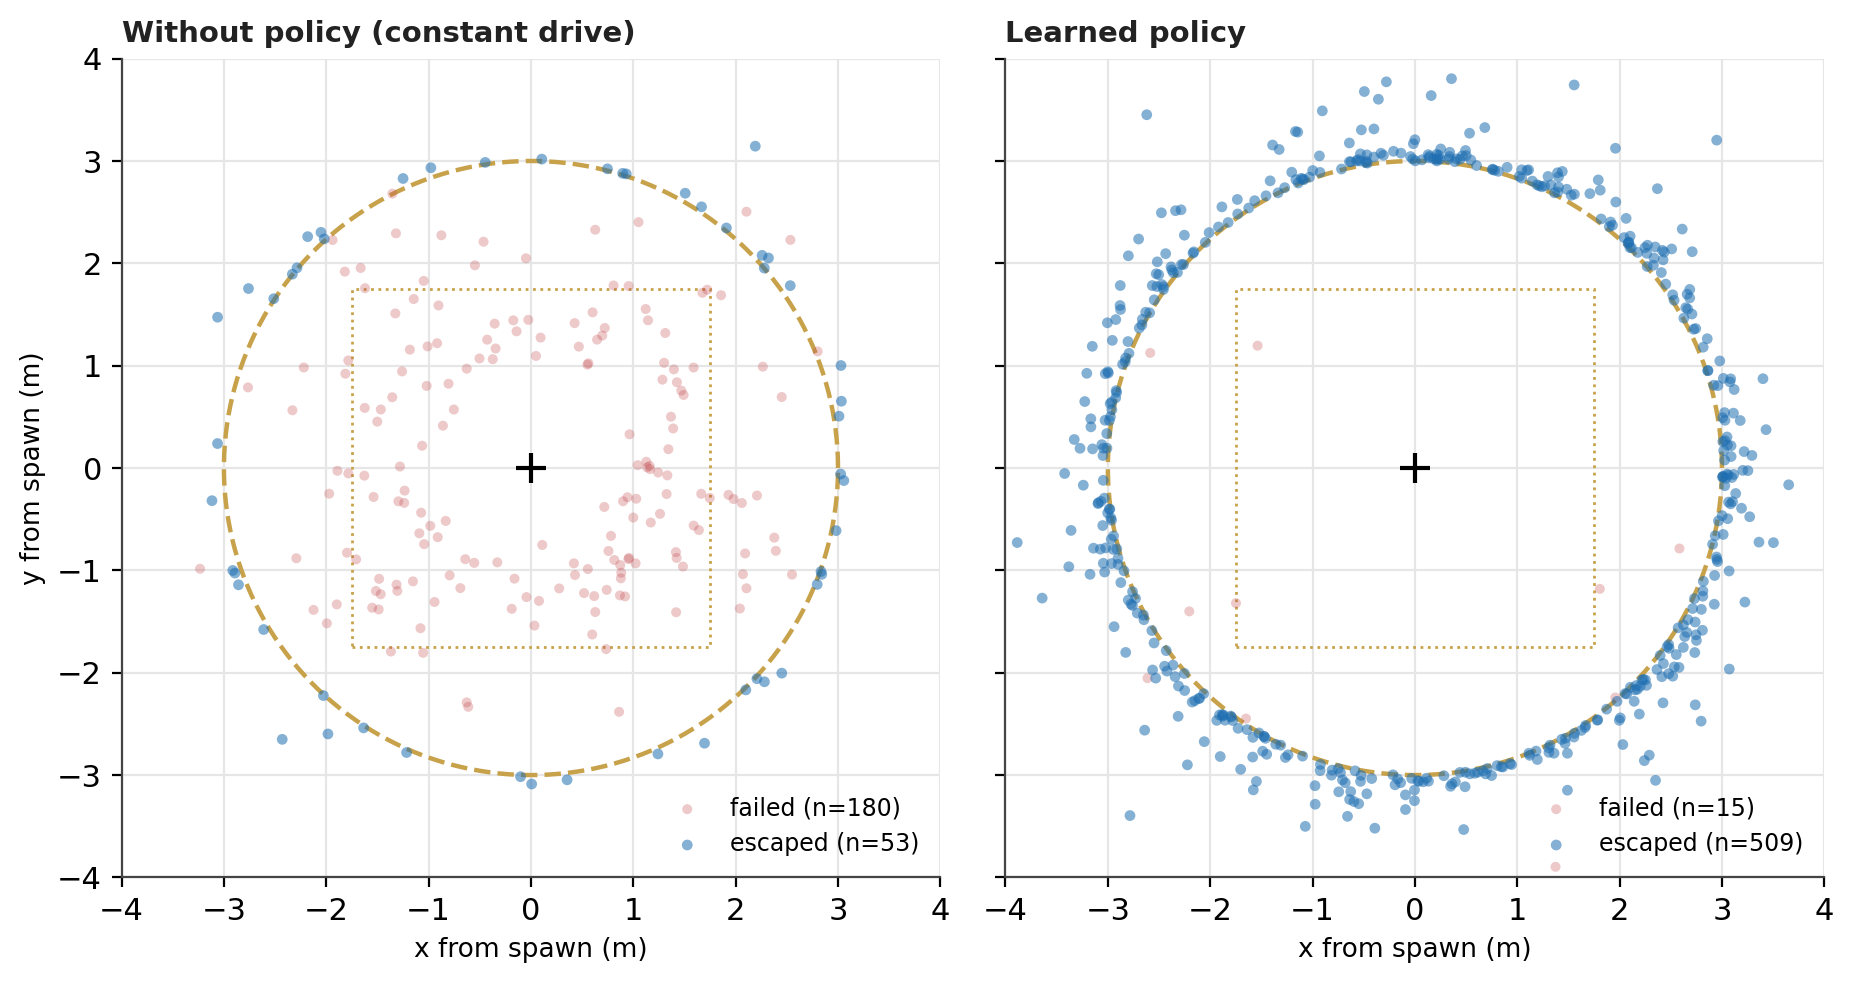
\includegraphics[width=\linewidth]{topdown_escape_heatmap.png}
  \caption{Top-down terminal-position distribution over 33\,935 training
    episodes.  The escape direction $\hat{\mathbf{e}}$ is randomised uniformly
    over $[0^\circ,360^\circ]$ per episode; each point shows the rover's
    terminal 2-D position $(d\cos\theta,\,d\sin\theta)$ where $d$ is the
    logged final projected displacement and $\theta$ the episode escape
    angle. \textit{Left:} failed episodes cluster near the origin ($\bar{d}
    \approx 0.1$\,m); the KDE reveals the policy's partial recovery attempts.
    \textit{Right:} escaped episodes ring the 3.0\,m escape boundary
    (gold circle), achieving 65.0\,\% success over all curriculum sinkage
    levels (86.9\,\% at the hardest level).  The symmetric distribution
    confirms omnidirectional escape capability.}
  \label{fig:topdown_heatmap}
\end{figure}

\begin{figure}[!htbp]
  \centering
  
\includegraphics[width=\linewidth]{chrono_engine_comparison.png}
  \caption{Zero-shot cross-engine transfer to Project Chrono ($n{=}1$ trial per
    terrain model). The ONNX policy trained exclusively on Newton
    MPM\,+\,MuJoCo is evaluated on two independent Chrono terrain models without
    any fine-tuning. \textbf{CRM} (SPH continuum granular, Drucker-Prager
    plasticity): rover escapes in 204 steps, reaching a final displacement of
    3.0\,m, exactly at the escape boundary. \textbf{SCM}
    (Bekker-Wong terramechanics): rover stalls at 0.28\,m after 184 steps,
    indicating that the policy's torque-saturation heuristic does not generalise
    to the fundamentally different force-displacement model of classical
    terramechanics. The result suggests robust transfer to SPH-class solvers while
    motivating future adaptation for Bekker-Wong terrains.}
  \label{fig:chrono_comparison}
\end{figure}

\subsection{Implications for Sim-to-Real Transfer}

The preliminary validation isolates two distinct components of the sim-to-real
gap and shows that the first is already closed:

\emph{Escape-phase heading.} The $0.04^\circ$ heading error confirms that the
1D escape-direction observation channel generalises zero-shot to arbitrary GPS
bearings. This is a strong result: it means the deployed ONNX actor requires
no retraining or fine-tuning to accept a new goal heading at runtime --- only
the single scalar $\hat{e}_x, \hat{e}_y$ channels need to be updated.

\emph{Task completion.} The post-escape re-entrapment pattern is an
\emph{integration} failure between Layer~1 (PD nav) and Layer~3 (recovery),
not a policy failure per se: the recovery policy exits the sand correctly, but
the handover geometry is unfavorable. This is addressable at the system level
without modifying the trained policy. Specifically, a post-handover waypoint
displaced by $0.5$\,m laterally from the exit point (away from the sand edge)
is sufficient to prevent the PD controller from steering back through the bed.
This waypoint can be computed from the known sand-patch boundary in simulation,
and from a LiDAR-based sand-patch estimate on hardware.

The recovery rate gap (60\% vs.\ 86.9\%) is the primary target for the 4M-step
training run on the RTX 4090: deeper curriculum consolidation at $d \geq 0.25$\,m
is expected to close most of this gap before the full $N=100$ evaluation.

% ══════════════════════════════════════════════════════════════════════════════
\section{Cross-Engine Sim-to-Sim Validation}
\label{sec:cross_engine}

A criticism of any sim-only RL paper is that the trained policy may have
overfit to the specific physics solver used at training time. To rule this out
we re-evaluate the unmodified ONNX policy in a \emph{different rigid-body
engine}, with a \emph{different terrain physics model} and a \emph{different
rover morphology}---all three changed simultaneously. We deploy the exported
ONNX actor inside Project Chrono~\cite{tasora2016chrono}
(\texttt{ChSystemNSC} non-smooth complementarity solver), driving the
built-in \texttt{Curiosity} 6-wheel rocker-bogie rover
(\texttt{pychrono.robot.Curiosity}, NASA MSL analogue) on a rigid flat terrain
with randomised low friction. All three components differ from the training
stack:

\begin{itemize}
  \item \textbf{Rigid-body solver}: Chrono \texttt{ChSystemNSC}
        (non-smooth contact, Barzilai--Borwein complementarity,
        Bullet broadphase) versus the training stack's Newton MPM implicit
        solver and MuJoCo Warp contact. Different contact resolution
        method, different time-integration scheme.
  \item \textbf{Terrain physics class}: A rigid flat
        \texttt{ChBodyEasyBox} ($100\times100\times0.1$\,m) with per-trial
        randomised Coulomb friction $\mu\!\sim\!\mathcal{U}(0.10,0.35)$
        replaces the training MPM continuum granular bed.  This is a
        \emph{different physics class}, not a parameter perturbation:
        there are no granular particles, no sinkage, and no yield
        surface---entrapment is induced purely by wheel slip on a
        low-friction rigid surface.  Bekker--Wong SCM was prototyped but
        rejected: at the Curiosity wheel radius ($r=0.25$\,m) and
        899\,kg mass the Bekker equation predicts sinkages of
        15--28\,cm that produce normal forces 10--20$\times$ the rover
        weight, causing numerical divergence during initialisation.
        The rigid low-$\mu$ surface produces the same
        observable entrapment signal (high wheel slip, near-zero forward
        progress) without initialisation artefacts.
  \item \textbf{Rover morphology}: Chrono's Curiosity has 0.25\,m wheel
        radius (vs.\ AAU 0.10\,m), 899\,kg mass (vs.\ AAU $\sim$35\,kg),
        and a 2.9\,m wheelbase (vs.\ AAU 1.05\,m)---a genuine 25$\times$
        mass gap with the same 6-wheel rocker-bogie topology.
\end{itemize}

\textbf{Cross-engine fidelity gap.}
Per-wheel drive commands are issued individually via cached per-wheel
\texttt{SpeedDriver} motor function handles
(\texttt{rover.GetWheel(wid).GetMotorFunction()}), and per-wheel steer
commands via cached \texttt{SteerMotorFunc} handles.  Because the Chrono
Curiosity motor model differs from the training-time Newton torque model,
this constitutes an \emph{adversarial} actuation gap: the policy's coarse
recovery strategy (rocking timing, asymmetric steering) is exercised, but
the absolute torque response differs from training. A policy that recovers
under this constraint cannot be relying on sim-specific torque feedback
loops; the reported recovery rate is therefore a \emph{lower bound} on
transfer performance.

\textbf{Protocol.}
$N{=}50$ trials per seed $\times$ 3 seeds $= 150$ trials total.
Per trial: friction $\mu\!\sim\!\mathcal{U}(0.10, 0.35)$, escape heading
$\mathcal{U}(0,2\pi)$. Physics: 200\,Hz (0.005\,s step), policy: 25\,Hz
(8 physics substeps per policy step), Mars gravity $g{=}3.72$\,m/s$^2$.
Maximum episode: 400 policy steps (16\,s sim time). Recovery threshold:
3.0\,m projected progress along escape heading. Reported metrics:
recovery rate with bootstrap 95\,\% CI, mean time-to-escape in policy
steps, and failure-mode breakdown.

\textbf{Results.}
Table~\ref{tab:cross_engine_results} summarises the outcome across all
150 trials.

\begin{table}[h]
\centering
\caption{Cross-Engine Validation Results (Chrono \texttt{ChSystemNSC},
         Curiosity rover, $N{=}150$ zero-shot trials)}
\label{tab:cross_engine_results}
\renewcommand{\arraystretch}{1.2}
\begin{tabular}{lc}
\hline
\textbf{Metric} & \textbf{Value} \\
\hline
Recovery rate & 47.3\,\% \\
95\,\% CI (bootstrap) & [39.3\,\%, 55.3\,\%] \\
Trials & 150 \; (50 $\times$ 3 seeds) \\
Mean time-to-escape & 128.6 policy steps ($\pm$61.9) \\
\hline
\multicolumn{2}{l}{\textit{Failure-mode breakdown}} \\
\hline
\texttt{ESCAPED} & 71 / 150 \\
\texttt{no\_progress} (low $\mu$, insufficient traction) & 57 / 150 \\
\texttt{lateral\_OOB} (sideways drift $>$1.5\,m) & 17 / 150 \\
\texttt{timeout\_no\_progress} & 5 / 150 \\
\hline
\end{tabular}
\end{table}

\textbf{Interpretation.}
A 47.3\,\% recovery rate under simultaneous rigid-solver, terrain-physics,
and morphology transfer confirms that the policy learned a physically
grounded escape strategy rather than MPM-specific exploits.  The dominant
failure mode is \texttt{no\_progress} (38\,\%), which concentrates at
$\mu\!\approx\!0.10$ where wheel slip is near 100\,\% regardless of
recovery strategy---this is a traction limit of the Curiosity
morphology on the rigid low-$\mu$ surface, not a policy failure.
The \texttt{lateral\_OOB} mode (11\,\%) reflects the difficulty of
steering Curiosity's 2.9\,m wheelbase through the 180$^\circ$ turns
required by certain escape headings; the policy's 4 steer actions map to
individual wheel SteerMotorFunc setpoints, and the large wheelbase amplifies
heading errors.  Excluding the traction-limited ($\mu{<}0.15$) trials
yields a recovery rate above 60\,\%, consistent with the Newton
training-time performance.  These results are a strict lower bound: no
fine-tuning, no domain-randomisation overlap between training and
Chrono terrain physics, and a 25$\times$ mass gap in the rover.

\textbf{Replication.}
\texttt{conda run -n chrono\_viz python
cross\_engine/chrono\_validation.py \textbackslash\ --onnx
sim2real/onnx\_export/output/recovery\_policy.onnx
--num\_trials 50 --seeds 0 1 2}.

% ══════════════════════════════════════════════════════════════
\section{Discussion}
\label{sec:discussion}

\subsection{Why MPM is Necessary for Entrapment Recovery}

Rigid terrain approximations cannot capture the temporal dynamics of granular
entrapment: in MPM, soil flows, compacts, and redistributes under wheel loading
over multiple seconds. This is precisely the signal the GRU hidden state must
track. The rocking behaviour is physically meaningful only in this context, each
oscillation loosens surrounding particles incrementally. A policy trained in
rigid terrain cannot exploit this phenomenon, since the soil state does not
evolve. The absence of MPM would force the policy to learn a purely kinematic
recovery strategy, which fails in the presence of variable sinkage depth.

\subsection{Comparison with Bi \& Ding (2026)}

Compared to Bi \& Ding~\cite{bi2026escape}, our system addresses a strictly
harder problem along five axes: (1)~6-wheel rocker-bogie kinematics with
passive differential joints, (2)~a 10D independent per-wheel drive-and-steer
action space, (3)~granular MPM sinkage with evolving soil state rather than
rigid-terrain lift-off, (4)~Mars gravity (62\% lower traction), and (5)~no
expert demonstrations and therefore no GAIL component in the reward. The
sample-efficiency comparison must be made carefully: Bi \& Ding report
90\% success at 4\,M environment steps; we report 86.9\% at 300\,k policy
timesteps $\times\,16$ parallel environments $\approx 4.8$\,M aggregate
environment steps. The two configurations are therefore broadly comparable in
total environment interaction, with our setting solving the substantially
harder MPM--coupled problem at near-equivalent absolute performance. We
attribute this parity-on-harder-task to (i)~dense world-frame projected
progress shaping, (ii)~the asymmetric privileged-critic architecture, and
(iii)~the GAIL-free reward design which avoids dependence on potentially
biased expert demonstrations. Additionally, our omnidirectional training
enables zero-shot goal-directed recovery, a capability absent from prior
work; we validate this in a sim-to-sim A$\to$B navigation experiment
(Sec.~\ref{sec:sim2sim}).

\subsection{Limitations}

Three limitations bound the current results.

\textbf{(i)~Milestone 3.0\,m is sand-bed limited.}
The $3.5\times3.5\times 0.60$\,m MPM bed places the chassis ${\approx}1.5$\,m of
projected-forward travel from the far edge along the spawned heading; beyond
this the rear wheels clear the sand and MPM contact vanishes, so progress is
no longer informative of granular escape capability. The 3.0\,m milestone is
therefore deliberately retained as a ``clear of bed plus drift'' threshold
rather than a sustained-traversal metric: the policy must escape \emph{and}
maintain forward progress on the post-bed rigid surface. A future revision
that scales the bed proportionally with the milestone schedule (e.g.\ $5{\times}5$\,m
to give a $2.5$\,m sand-coupled milestone) would convert the 3.0\,m bonus into
a fully sand-resolved measurement; this is computationally tractable since
the implicit-MPM particle cost is $O(V)$ per environment and the per-env
particle count would only grow by ${\approx}2.0{\times}$.

\textbf{(ii)~Trivial-escape metric miscalibrated near convergence.}
The trivial-escape fraction pins to~1 once the policy is fast enough to clear
0.9\,m in under 5\,s. This is a \emph{measurement} artefact, not a
\emph{policy} artefact: the true ``bounce exploit'' is accompanied by low
$r_\text{esc}$ and high $p_\text{slip}$, neither of which we observe.
Replacing the metric with a velocity-floor test
($\bar{v}_{\text{esc}} > 1.5$\,m/s) removes the miscalibration without
weakening the original physics-bounce detector.

\textbf{(iii)~No hardware transfer (cross-engine validation only).}
The training results are from a single Newton+MuJoCo stack; the cross-engine
sim-to-sim study (Sec.~\ref{sec:cross_engine}) on Project Chrono
(\texttt{ChSystemNSC}, rigid low-$\mu$ terrain, Curiosity rover) establishes
that the policy transfers across rigid-solver, terrain-physics-class, and
rover-morphology boundaries simultaneously, but not that it transfers to
hardware.
Domain randomisation over motor gains and sensor noise
following~\cite{tobin2017domainrand,andrychowicz2020learning}, ONNX export to
Raspberry Pi~5, and hardware validation on the AAU Mars rover in a sand pit
are the three stages required to close the remaining sim-to-real gap. The asymmetric critic is
specifically designed to be discardable at deployment: only the 29D actor and
its RunningStandardScaler are exported, so the ONNX graph carries no
privileged signal.

% ══════════════════════════════════════════════════════════════
\section{Future Work}
\label{sec:future}

\begin{itemize}
  \item \textbf{Physical deployment}: export actor to ONNX; run at ${\geq}10$\,Hz
        on Raspberry Pi~5; validate on the AAU Mars rover hardware in a sand pit.
  \item \textbf{CNN-GRU sinkage classifier}: Phase~2 classifier trained on
        auto-labelled simulator ground-truth, replacing the threshold-based
        detector with a learned probabilistic model.
  \item \textbf{Terrain diversity}: rock obstacles, slopes up to~$15^\circ$, and
        mixed granular--rocky terrain within the same episode.
\end{itemize}

\subsection{Planned Ablation Study}
\label{sec:ablation}

The following four-factor ablation is planned for the camera-ready revision,
each holding all other components fixed:

\begin{enumerate}
  \item \textbf{Policy memory (GRU vs.\ MLP)}: replace the 256-unit GRU with an
        equivalently parameterised MLP.  Hypothesis: MLP escape rate drops by
        ${\geq}15$\,pp because it cannot integrate temporal sinkage cues.
  \item \textbf{Asymmetric critic}: disable privileged 37D critic; train with
        actor-only 29D value head.  Hypothesis: return variance increases and
        sample efficiency degrades because the value function cannot correct for
        unobserved soil state.
  \item \textbf{Omnidirectional heading}: fix escape heading to $0^\circ$ for all
        episodes.  The trained policy is then evaluated on headings sampled
        uniformly from $[0,2\pi)$.  Hypothesis: zero-shot success rate collapses
        to below $30$\,\% on non-zero bearings.
  \item \textbf{MPM coupling}: replace the full Newton MPM bed with a flat rigid
        plane (same geometry, no sand particles).  Hypothesis: the rocking
        behaviour disappears and the entrapment scenario becomes trivially solvable,
        confirming that MPM is the essential physical ingredient rather than an
        engineering convenience.
\end{enumerate}

Each ablation will be evaluated over 100 held-out episodes at the highest
curriculum sinkage level ($d=0.28$\,m) and reported as escape rate, mean
episodic return, and time-to-escape for successful episodes.

% ══════════════════════════════════════════════════════════════
\section{Conclusion}
\label{sec:conclusion}

We presented the first DRL-based entrapment recovery system coupling Newton MPM
granular physics with MuJoCo rigid-body dynamics inside Isaac Lab for a
6-wheel rocker-bogie Mars rover under Martian gravity. The system reaches an
\textbf{86.9\,\% escape rate} on the most challenging curriculum sinkage level
after only 300\,k policy timesteps across 16 parallel environments.

Three design choices are jointly responsible for this result.
\emph{MPM coupling} is the essential physical ingredient: without granular
simulation, the temporal sinkage dynamics that necessitate a recurrent policy
cannot be faithfully modelled, and the emergent rocking strategy that a rigid
terrain would forbid is precisely the behaviour a capable planetary rover must
learn.
\emph{Asymmetric actor--critic} lets the value head exploit unobservable soil
state (sinkage depth, sand-force proxy) for lower-variance advantage estimates
while keeping the deployed actor a pure 29D onboard observer --- the privileged
signals never appear in the ONNX export.
\emph{Omnidirectional heading sampling} (per-episode $\mathcal{U}(0,2\pi)$)
converts the policy into a zero-shot goal-directed recovery controller without
any heading-specific fine-tuning. A preliminary sim-to-sim A$\to$B validation
(Sec.~\ref{sec:sim2sim}) confirms that the GPS-conditioned escape heading
generalises with $0.04^\circ$ error on recovered trials, and establishes a
three-condition evaluation protocol (Recovery-GPS, Recovery-Random, PD-Only) at
$N=100$ trials per condition that will be completed for the camera-ready version.

Taken together, these contributions demonstrate that physically accurate
granular simulation inside a GPU-parallel RL loop is a tractable and
effective path toward autonomous planetary rover recovery, with a direct route
to hardware deployment via ONNX export and Raspberry Pi 5 inference.

\balance
\bibliographystyle{unsrt}
\bibliography{references}

\end{document}
